%!TeX program = xelatex
%!TeX builder = latexmk

%模板
\documentclass[10pt,a4paper,twoside]{book}

\usepackage{ctex}
\usepackage{makecell}
\usepackage{enumerate}%罗列专用宏包
\usepackage{graphicx}%插入图片的宏包
\usepackage{subfigure}
\usepackage{newtxtext}
\usepackage{newtxmath}
\usepackage{bm}
\DeclareMathSizes{10}{10}{5.5}{4}
\usepackage{makeidx}%索引专用
\makeindex  %添加索引
\usepackage{fancyhdr}
%\usepackage{textcomp}%树叶图案在这个包里
%\usepackage{bbding}%很多漂亮的图案
\usepackage[dvipsnames, svgnames, x11names]{xcolor}%导入了所有颜色配置文件的宏包
\usepackage{geometry}%页边距调整
\geometry{left=2cm,right=2cm,bottom=2cm,top=2cm}
\usepackage{titletoc}%目录页的宏包
\usepackage{titlesec}%改变章节或标题的样式的宏包
\usepackage[bookmarks=true,colorlinks,linkcolor=black]{hyperref}
\usepackage{enumerate}%使用改宏包优化罗列环境
\usepackage{tcolorbox}%box宏包
\tcbuselibrary{most}
\usepackage{xcolor}
\usepackage{colortbl,booktabs}%第二个包定义了几个*rule  
\usepackage{multicol}
\usepackage{multirow}
\usepackage{tikz}
\usepackage{capt-of}
\usepackage{mhchem}
\usepackage{lipsum}
%\usepackage{longtable}
%\usepackage{polynom}% 除法竖式
\usetikzlibrary{shapes.geometric}
\usetikzlibrary{arrows,arrows.meta}
\tikzstyle{arrow} = [thick,->,>=stealth]
%\usetikzlibrary{circuits.ee.IEC}

%字体设置
\setCJKmainfont[BoldFont={PingFangSC-Medium}]{PingFangSC-Regular}

%章节或标题的样式
\titleformat{\chapter}{\bfseries\Huge\color{titlepurple}}{第\ \thechapter\ 章\ \quad}{0pt}{}
\titleformat{\section}{\Large\color{titlepurpleb}}{\bfseries{\thesection}\quad  }{0pt}{}
\titleformat{\subsection}{\large\color{titlepurplec}}{\bfseries{\thesubsection}\quad  }{0pt}{}
\titlespacing{\subsection}{1.5em}{0.1em}{1em}[1em]
%格式如下:\titlespacing*{章节名称}{左间距}{(前)行间距}{(后)行间距}[右间距(一般都没用,填0.1em即可,但不能不填)]
\titlespacing*{\subsubsection}{2em}{3em}{1em}[1em]

%目录调整
\newcounter{mycontents}
\newcommand{\thecontents}{\refstepcounter{mycontents} \alph{mycontents}.}
%\titlecontents{标题名}[左间距]{标题格式}{标题标志}{无序号标题}{指引线与页码}[下间距]
\titlecontents{chapter}
[0cm]
{\bf \large \vspace{0.8em} }{\contentspush{第 \thecontentslabel\ 章 \hspace*{0.8em}}}{}{\titlerule*[0.5pc]{$\cdot$}\contentspage}
\titlecontents{section}[1.7cm]{\bf  \vspace{0.5em} }{\contentslabel{2.4em}}{\hspace*{-2.5em} \thecontents \hspace*{0.8em}}{\titlerule*[0.5pc]{$\cdot$}\contentspage}
\titlecontents{subsection}[2.5cm]{\small \vspace{0.2em} }{\contentslabel{3em}}{}{\titlerule*[0.5pc]{$\cdot$}\contentspage}

%定义颜色
%定义某个颜色,对应颜色代号查表
\definecolor{titlepurple}{HTML}{5758BB}%一级标题(目前:蓝紫色)
\definecolor{titlepurpleb}{HTML}{3A006F}%二级标题(目前:深紫色)
\definecolor{titlepurplec}{HTML}{006266}%三级标题(目前:墨绿色)
\definecolor{tab1}{HTML}{9698ED}%表格1
\definecolor{tab2}{HTML}{DBDCFF}%表格2
\definecolor{dy0}{HTML}{EA7500}%小标题定义专用(目前:橙黄色)
\definecolor{dl}{HTML}{007500}%小标题定理专用(目前:深绿色)
\definecolor{inference}{HTML}{343300}%小标题推论专用(目前:墨绿色)
\definecolor{ex}{HTML}{7158e2}%小标题例专用(目前:紫色)
\definecolor{dy}{HTML}{BF0060}%夹杂在文本中的定义词的颜色1(目前:深红色)
\definecolor{dy2}{HTML}{FF0000}%夹杂在文本中的定义词的颜色2(目前:红紫色)
\definecolor{dya}{HTML}{FFFFFF}
\definecolor{超链接}{HTML}{0000C6}%含超链接的文字专用色(目前:蓝紫色)
\definecolor{文字底色}{HTML}{F8FF00}%强调的文字底色(目前:黄色)
\definecolor{eq}{HTML}{F0F0F0}
\definecolor{tl}{HTML}{D94600}


%定义计数器
\newcounter{theorem}[chapter]
\newcounter{defination}[chapter]
\newcounter{example}[chapter]
\newcounter{inference}[chapter]
\newcounter{examples}[chapter]
\newcounter{tl}[chapter]
\newcounter{F}[section]
\newcounter{G}[section]
\newcounter{H}[section]
\renewcommand{\thetheorem}{{ 定理} \textbf{\thechapter.\arabic{theorem}}}
\renewcommand{\thedefination}{{ 定义} \textbf{\thechapter.\arabic{defination}}}
\renewcommand{\theexample}{{ 题型} \textbf{\thechapter.\arabic{example}}}
\renewcommand{\theinference}{{ 方法} \textbf{\thechapter.\arabic{inference}}}
\renewcommand{\theexamples}{{ 例}  \textbf{\thechapter.\arabic{examples}}}
\renewcommand{\thetl}{{ 推论}  \textbf{\thechapter.\arabic{tl}}}
\newcommand{\sj}{\hspace*{-2.7em}}

%定义环境
\newcommand{\mybox}[2][]{
	\begin{tcolorbox}[on line,
		arc=0pt,outer arc=0pt,colback=#1!10!white,colframe=#1,
		boxsep=0pt,left=3pt,right=3pt,top=6pt,bottom=6pt,
		boxrule=0pt,leftrule=1.5pt]#2
\end{tcolorbox}}

%定理类
\newcommand{\theorem}[2][]{\vspace{1em}\sj \refstepcounter{theorem} \mybox[dl]{{\color{dl}\thetheorem\hspace{1em}#1}\\[0.1em] \hspace*{2em}#2}\vspace{0.5em}  \par}

%推论类
\newcommand{\inference}[2][]{\vspace{1em}\sj \refstepcounter{inference} \mybox[inference]{{\color{inference}\theinference\hspace{1em}#1}\\ \hspace*{1.5em}#2}\vspace{0.5em}   \par}

%定义类
\newcommand{\defination}[2][]{\vspace{1em}\sj \refstepcounter{defination} \mybox[dy0]{{\color{dy0}\thedefination\hspace{1em}#1}\\[0.1em] \hspace*{2em}#2}\vspace{0.5em} \par}

%题型类(无标签)
\newcommand{\example}[1][]{\vspace{1em} \sj \refstepcounter{example} \mybox[ex]{\color{ex}\theexample\hspace{1em}#1}\vspace{0.5em} \par }


%调整间距(倍数)
\linespread{1.5}

%自定义页眉页脚---------------
\pagestyle{fancy}
\renewcommand{\chaptermark}[1]{\markboth{\;第\ \thechapter\ 章\quad#1\;}{}}
\renewcommand{\sectionmark}[1]{\markright{\;\thesection\ #1\;}}
\fancyhf{}
%\fancyfoot[C]{\bfseries\thepage}
\fancyhead[LO]{\small\CJKfamily{song}\rightmark}
\fancyhead[RE]{\small\CJKfamily{song}\leftmark}
\fancyhead[RO,LE]{\;\thepage\;}
\fancyfoot[RO,LE]{\footnotesize\CJKfamily{heilight}{火箭推进理论}}
\fancyfoot[RE,LO]{\footnotesize\CJKfamily{heilight}Rocket Propulsion Theory}
\renewcommand{\headrulewidth}{0.4pt} % 注意不用\setlength
%\renewcommand{\footrulewidth}{0pt}
\fancyheadoffset[LE,RO]{0cm}
\fancyfootoffset[LE,RO]{0cm}
% 注意不用\setlength
%\renewcommand{\footrulewidth}{0pt}


%自定义命令
%% 文本设置类
\newcommand{\link}[1][]{\hyperref[#1] {\color{超链接}#1}}
\newcommand{\ds}[1][]{\colorbox{文字底色}{#1}}
\newcommand{\red}[1][]{\textcolor{red}{#1}}
\newcommand{\blue}[1][]{\textcolor{blue}{#1}}
\newcounter{sssection}[subsection]
\newcommand{\sssection}[1][]{\noindent \refstepcounter{sssection} \textbf{\thesssection. #1} \vspace*{0.5em}}

%% 公式字符类
\renewcommand{\d}{{\rm{d}}}
\newcommand{\e}{{\rm{e}}}
\newcommand{\n}{{\rm{n}}}
\renewcommand{\a}{\text{a}}
\renewcommand{\c}{\text{c}}
\renewcommand{\t}{\text{t}}
\renewcommand{\j}{\text{j}}
\def\degree{{}^{\circ}}
\newcommand{\hvdots}{\hspace*{2mm}\vdots\hspace*{2mm}}
\newcommand{\RMn}[1][]{\romannumeral#1}
\newcommand{\RMN}[1][]{\uppercase\expandafter{\romannumeral#1}}
\newcommand{\vi}{\bm{i}}
\newcommand{\vj}{\bm{j}}
\newcommand{\vk}{\bm{k}}
\newcommand{\f}{\text{f}}
\newcommand{\s}{\text{s}}
\newcommand{\st}{\text{st}}

%% 定义索引类
\newcommand{\dy}[2][]{{\color{dy}#1}\index{#2@#1}}
\newcommand{\dya}[2][]{\vspace*{0.7em} \noindent \tcbox[colframe =Chocolate , colback =Coral,boxrule=0.5mm,size=small,on line]{\color{dya}{\textbf{#1}}}  \index{#2@#1} \hspace*{1em}}
\newcommand{\dyb}[1][]{\vspace*{0.7em} \noindent \tcbox[colframe =Chocolate, colback =Coral,boxrule=0.5mm,size=small,on line]{\color{dya}{\textbf{#1}}} \hspace*{1em} }


%--------------------------------------------------------图框定义---------------------------------------------------------%
%证明和解
\newcommand{\proof}{\vspace*{1em} \noindent  \hspace*{0.2em}  \tcbox[colframe =black, colback =black!10!white,boxrule=0.5mm,size=small,on line]{\color{black}{{ 证}}}\hspace{1.5em}}
\newcommand{\solve}{\vspace*{1em} \noindent  \hspace*{0.2em}  \tcbox[colframe =black, colback =black!10!white,boxrule=0.5mm,size=small,on line]{\color{black}{{ 解}}\hspace*{0.25em}}\hspace{1.5em}}
\newcommand{\solveother}{\vspace*{1em} \noindent  \hspace*{0.2em}  \tcbox[colframe =black, colback =black!10!white,boxrule=0.5mm,size=small,on line]{\color{black}{{ 另解}}}\hspace{1.5em}}
\newcommand{\errsolve}{\vspace*{1em} \noindent  \hspace*{0.2em}  \tcbox[colframe =red, colback =red!10!white,boxrule=0.5mm,size=small,on line]{\color{red}{{ 错解}}}\hspace{1.5em}}
\newcommand{\errreason}{\vspace*{1em} \noindent  \hspace*{0.2em}  \tcbox[colframe =red, colback =red!10!white,boxrule=0.5mm,size=small,on line]{\color{red}{{ 错因}}}\hspace{1.5em}}
\newcommand{\solvereason}{\vspace*{1em} \noindent  \hspace*{0.2em}  \tcbox[colframe =ForestGreen
	, colback =ForestGreen!15!white,boxrule=0.5mm,size=small,on line]{\color{ForestGreen}{{ 解析}}}\hspace{1.5em}}

%例
\newcommand{\examples}{\vspace*{1em}\noindent  \refstepcounter{examples} \tcbox[colframe =ex, colback =ex!10!white,boxrule=0.5mm,size=small,on line]{\color{ex}{\theexamples}\hspace*{0.3em}}\hspace{1.5em}}
\newcommand{\simpleexamples}{ \noindent  \tcbox[colframe =ex, colback =ex!10!white,boxrule=0.5mm,size=small,on line]{  \color{ex}{例}}\hspace{1.5em}}

%推论
\newcommand{\tl}{\vspace*{1em}\noindent \refstepcounter{tl} \tcbox[colframe =tl, colback =tl!10!white,boxrule=0.5mm,size=small,on line]{\color{tl}{\thetl}\hspace*{0.3em}}\hspace{1.5em}}

%注意
\newcommand{\warn}[1][]{
	\vspace*{0.5em}
	\begin{tcolorbox}[colframe=red!75!black, colback=yellow!10!white,title=注意,fonttitle = ]
		#1
\end{tcolorbox}}
\newcommand{\summarize}[1][]{
	\vspace*{0.5em}
	\begin{tcolorbox}[colframe=white!20!black, colback=white!98!black,title=评注,fonttitle = ]
		#1
\end{tcolorbox}}

% 无编号索引
\newcommand\blfootnote[1]{% 
	\begingroup 
	\renewcommand\thefootnote{}\footnote{#1}% 
	\addtocounter{footnote}{-1}% 
	\endgroup 
}

%文本高亮
\newcommand{\highlights}[1][]{\tcbox[colframe =Chocolate , colback =Coral,boxrule=0.5mm,size=small,on line]{\color{white}{#1}}}

\title{
	\Huge{\textbf{火箭推进理论}}
	\vspace*{18em}
}
\author{
	{  \large {易鹏}}\\
	{  \large 中山大学}\vspace*{0.5em}\\
	内部版本号:V0.01.001$\,\,$(内测版)\\
}
%------------------------------------------------------------------------------------------------------------------------%

%文档开始
\begin{document}
	%标题及目录
	\pagenumbering{Roman}
	\maketitle
	\clearpage \phantom{s} \thispagestyle{empty} \clearpage
	\setcounter{page}{1}
	\tableofcontents
	
	%正文部分
	\cleardoublepage
	\setcounter{page}{1}
	\pagenumbering{arabic}
	
	\chapter{随机事件}
\thispagestyle{empty}
\section{随机事件}
\subsection{随机现象}
\dy[确定性现象]{QDXXX}
在一定条件下必然出现的结果\jg\\
\dy[随机现象]{SJXX}
事先无法准确与之其结果的现象\jg
\subsection{随机现象的统计性规律}
\dy[统计规律性]{TJGLX}
随机现象在大量重复出现时所表现出来的规律性.\jg\\
\dy[随机试验]{SJSY}
对随机现象的观察.\jg\\
\dya[随机试验的特点]
\begin{enumerate}[1.]
	\setlength{\itemindent}{3em}
	\setlength{\topsep}{0.01em}
	\setlength{\itemsep}{0.01em}
	\item 可重复性
	\item 可观察性
	\item 随机性
\end{enumerate}


\subsection{样本空间}
\dy[样本点]{YBD}
随机试验的每一个可能结果.\jg\\
\dy[样本空间]{YBKJ}
样本点的全体.\jg

\subsection{随机事件}
\dy[事件]{SJ}
实验结果具备的某一可观察的特征.\jg\\
\dy[随机事件]{SJSJ}
在随机试验中可能发生也可能不发生.\jg\\
\dy[必然事件]{BRSJ}
在试验中必然发生.\jg\\
\dy[不可能事件]{BKNSJ}
在试验中一定不发生.\jg\\
\dy[基本事件]{JBSJ}
对应一个唯一的可能结果,即样本点.\jg

\subsection{事件的集合表示}

\subsection{事件建的关系和运算}
\dy[事件的包含]{SJDBH}
$A$发生必然导致$B$发生,则称事件$B$包含事件$A$,记作$B\supset A$或$A\subset B$.\jg\\
\dy[事件的相等]{SJDXD}
事件$A$包含事件$B$,事件$B$也包含事件$A$,则称事件$A$与$B$相等,记作$A=B$.\jg\\
\dy[事件的并(或和)]{SJDB}
``事件$A$与$B$至少有一个发生"这一事件称为事件$A$和$B$的并(或和),记作$A\cup B$或$A+B$.\jg\\
\dy[事件的交(或积)]{SJDJ}
``事件$A$与$B$都发生"这一事件称为事件$A$与$B$的交(或积),记作$A\cap B$.\jg\\
\dy[事件的差]{SJDC}
``事件$A$发生而$B$不发生"这一事件称为事件$A$和$B$的差,记作$A-B$.\jg\\
\dy[互不相容事件]{HBXRSJ}
若事件$A$与$B$不能同时发生,也就是说$AB$时不可能事件,即$AB=\varnothing$,则称事件$A$与$B$是不可能事件.\jg\\
\dy[对立事件]{DLSJ}
``事件$A$不发生"这一事件称为事件$A$的对立事件,记作$\overline{A}$,易见,$\overline{A}=\Omega -A$,且$\overline{(\overline{A})}$.\jg\\
\dya[有限个事件的并与交]\jg
\newpage 
\noindent\dy[完备事件组]{WBSHZ}
\par 完备事件组设$A_1,A_2,\cdots,A_n,\cdots$是有限或可数个事件,如果其满足
\par \quad (1)  $A_iA_j=\varnothing,i\ne j,\quad i,j=1,2,\cdots $
\par \quad (2)  $\bigcup\limits_iA_i=\Omega$
\par 则称$A_1,A_2,\cdots,A_n,\cdots$是一个完备事件组.\jg\\
\dya[事件的关系与运算的文氏图]\jg

\subsection{随机事件的运算律}
\dya[求和运算]\jg
\par \quad 交换律
\begin{equation}
A \cup B =B \cup A
\end{equation}
\par \quad 结合律
\begin{equation}
(A \cup B)\cup C =A\cup (B\cup C)=A\cup B\cup C
\end{equation}
\dya[求交运算]\jg
\par \quad 交换律
\begin{equation}
A\cap B=B\cap A
\end{equation}
\par \quad 结合律
\begin{equation}
(A \cap B)\cap C=A\cap (B\cap C)=A \cap B \cap C
\end{equation}
\dya[混合运算]\jg
\par \quad 第一分配律
\begin{equation}
A \cap (B \cup C)=(A\cap B)\cup (A \cap C)
\end{equation}
\par \quad 第二分配律
\begin{equation}
A \cup (B \cap C)=(A\cup B)\cap (A \cup C)
\end{equation}
\dya[求对立事件的运算]\jg
\par \quad 自反律
\begin{equation}
\overline{(\overline{A})}=A
\end{equation}
\dya[求和及交事件的对立事件]\jg
\par \quad 第一对偶律
\begin{equation}
\overline{A \cup B}=\overline{A} \cap \overline{B} 
\end{equation}
\par \quad 第二对偶律
\begin{equation}
\overline{A \cap B}=\overline{A} \cup \overline{B} 
\end{equation}

\section{随机事件的概率}
\subsection{概率及其频率解释}
参见$\rm{P}_9$
\subsection{从频率的性质看概率的性质}
参见$\rm{P}_{10}$
\subsection{概率的公理化定义}
\sj
\defination[概率公理化]
设$\Omega $是一个样本空间,定义在$\Omega $的事件域$F$上的一个实值函数$P(\cdot)$如果它满足下列三条公理:
\begin{enumerate}[1.]
	\setlength{\itemindent}{4em}
	\setlength{\topsep}{0.01em}
	\setlength{\itemsep}{0.01em}
	\item $P(\Omega )=1$
	\item 对任意事件$A$,有$P(A) \le 0$
	\item 对任意可数的两两不相容的事件$A_1,A_2,\cdots,A_n,\cdots$,有$\displaystyle P\left( \bigcup_{i=1}^{\infty } A_i\right)=\sum_{i=1}^{\infty }P(A_i) $
\end{enumerate}
则称实值函数$P(\cdot)$为$\Omega $上的一个概率测度.\jg

\subsection{概率测度的性质}
\begin{enumerate}[1.]
	\setlength{\itemindent}{4em}
	\setlength{\topsep}{0.01em}
	\setlength{\itemsep}{0.01em}
	\item $P(\varnothing)=0$
	\item 有限可加性:$\displaystyle P\left( \bigcup_{i=1}^{\infty } A_i\right)=\sum_{i=1}^{\infty }P(A_i) $
	\item $P(\overline{A})=1-P(A)$
	\item $P(A-B)=P(A)-P(AB)=P(B)-P(AB)$
	\item $0\le P(A) \le 1$
	\item $P(A\cup B)=P(A)+P(B)-P(AB)$
\end{enumerate}

\section{古典概型与集合概型}
\subsection{古典概型}
\tdefination[古典概型]
古典概型是满足下面两个假设条件的概率模型:
\begin{enumerate}[1.]
	\setlength{\itemindent}{4em}
	\setlength{\topsep}{0.01em}
	\setlength{\itemsep}{0.01em}
	\item 随机试验只有有限个结果
	\item 每一个可能记过发生的概率相同
\end{enumerate}
所以,古典概型的概率测度可表述为:
\begin{equation}
P(A)=\frac{A\mbox{中的元素个数}}{\Omega \mbox{中的元素个数}}=\frac{\mbox{使}A\mbox{发生的基本事件数}}{\mbox{基本事件总数}}
\end{equation}

\subsection{几何概型}
\tdefination[几何概型]
几何概型的概率测度可表述为
\begin{equation}
P(A)=\frac{S(A)}{S(\Omega)}
\end{equation}

\section{条件概率}
\subsection{条件概率的定义}
\tdefination[条件概率]
给定概率空间$\Omega,P$,$A,B$是其上的两个事件,且$P(A)>0$,则称$\displaystyle P(B|A)=\frac{P(AB)}{P(A)}$为已知事件$A$发生的条件下,事件$B$发生的条件概率.

\subsection{乘法公式}
\ttheorem[乘法公式]
乘法公式的两个形式:
\begin{equation}
P(AB)=P(A)\cdot P(B|A),\,P(A)>0
\end{equation}
\begin{equation}
P(AB)=P(B)\cdot P(A|B),\,P(B)>0
\end{equation}

\subsection{全概率公式}
\ttheorem[全概率公式]
设$\lbrace A_i \rbrace$是一列有限或可数无穷个两两不相容的非零概率事件,且$\bigcup\limits_{i}A_i=\Omega $,则对任意事件$B,P(B)>0$,有
\begin{equation}
P(B)=\sum\limits_{i}P(A_i)\cdot P(B|A_i)
\end{equation}

\subsection{贝叶斯公式}
\ttheorem[贝叶斯公式]
设$\lbrace A_i \rbrace$是一列有限或可数无穷个两两不相容的非零概率事件,且$\bigcup_{i=1}^{\infty}A_i=\Omega $,则对任意事件$B,P(B)>0$,有
\begin{equation}
P(A_i|B)=\frac{P(A_iB)}{P(B)}=\frac{P(A_i)\cdot P(B|A_j)}{\sum\limits_{j}P(A_j)\cdot P(B|A_j)}
\end{equation}

\section{事件的独立性}
\subsection{两个事件的独立性}
\dy[两个事件的独立性]{LGSJDDLX}
如果$P(AB)=P(A)P(B)$,则称$A$与$B$相互独立,简称$A$与$B$独立.\jg\\
\dy[有限个事件的独立性]{YXGSJDDLX}
(1)  如果有$n(n\le 2)$个事件:$A_i,A_2,\cdots,A_n$中任意两个使劲按均相互独立,即对任意$1\le i\le j \le n$,均有$P(A_iA_j)=P(A_i)P(A_j)$,则称$n$个事件$A_i,A_2,\cdots,A_n$两两独立.
\par (2)  设$A_i,A_2,\cdots,A_n$为$n(n\le 2)$个事件,如果对其中任何$k(2\le k\le n)$个事件$A_{i_1},A_{i_2},\cdots,A_{i_k}\,(1 \le i_1<i_2<\cdots<i_k\le n)$,均有$P(A_{i_1}A_{i_2}\cdots A_{i_k})=P(A_{i_1})P(A_{i_2})\cdots P(A_{i_k})$,则称
事件$A_i,A_2,\cdots,A_n$为$n(n\le 2)$相互独立.

\subsection{相互独立性的性质}
\ttheorem[相互独立性的性质]
1.  如果$n$个事件$A_1,A_2,⋯,A_n$相互独立,则将其中任何$m(1\leq m \leq n)$个事件改为相应的对立事件,形成的新的$n$个事件仍然相互独立.
\par 2.  如果$n$个事件$A_1,A_2,⋯,A_n$相互独立,则有
\begin{equation}
	P\left( \bigcup_{i=1}^{n} A_i\right) =1-\prod_{i=1}^{n}P\left(\overline{A_i} \right) =1-\prod_{i=1}^{n}\left[1- P\left(A_i \right)\right]
\end{equation}

\subsection{伯努利概型}
\tdefination[伯努利概型]
只有两个可能的结果的试验称为伯努利试验,一个伯努利试验独立重复$n$次形成的试验序列称为$n$重伯努利试验.
\jg

\theorem[伯努利定理]
在一次试验中,事件$A$发生的概率为$p(0<p<1)$,则在$n$重伯努利试验中,事件$A$恰好发生$k$次的概率$b(k;n,p)$为
\begin{equation}
b(k;n,p)=C_n^k\,p^k\,q^{n-k}
\end{equation}
其中,$q=1-p.$
\par 在伯努利试验序列中,设每次试验中事件$A$发生的概率为$p$,“事件$A$在第$k$次试验中才首次发生”$(k≥1)$这一事件的概率为
\begin{equation}
g(k,p)=p\,q^{k-1}
\end{equation}




	
	\chapter{热力学第一定律}
\thispagestyle{empty}
\section{能量守恒概述}
\ttheorem[能量守恒定律]
自然界一切物质具有能量,能量既不能凭空创造,也不能自我消灭,而只能在一定条件下从一种形式转换为另一种形式,或从一个物体传递到另一个物体。在转换和传递的过程中,能量的总量恒定不变。\index{NLSHDL@能量守恒定律}

\begin{itemize}
	\item 能量的不同形式:能量的转换
	\item 能量的不同载体:能量的传递 
\end{itemize}

\section{热力学第一定律的总体方程}
针对热力系统,应用能量守恒,有
\begin{equation}
	\mbox{系统输入能量}-\mbox{系统输出能量}=\mbox{系统能量的增量}
\end{equation}
考虑系统与外界能量传递的三条途径:
\begin{itemize}
	\item 热量传递:通过传热的形式传递热量$Q$;
	\item 功量传递:通过作功的形式传递能量$W$;
	\item 因质量传递而带入或带出能量$\psi$。
\end{itemize}
可以得到
\begin{equation}
	\left(Q_{\mbox{\tiny 入}}+W_{\mbox{\tiny 入}}+\varPsi_{\mbox{\tiny 入}}\right)\,-\,\left(Q_{\mbox{\tiny 出}}+W_{\mbox{\tiny 出}}+\varPsi_{\mbox{\tiny 出}}\right) = \Delta E
\end{equation}
记$Q = Q_{\mbox{\tiny 入}}-Q_{\mbox{\tiny 出}}, \, W = W_{\mbox{\tiny 入}} -W_{\mbox{\tiny 出}}, \, \varPsi_2 = \varPsi_{\mbox{\tiny 出}}, \, \varPsi_1 = \varPsi_{\mbox{\tiny 入}}$,则有
\begin{equation}
	Q = \Delta E + W + (\varPsi_2 - \varPsi_1) 
	\label{热一总体方程}
\end{equation}

\begin{itemize}
	\item $Q,W$符号的意义
	\begin{itemize}
		\item $Q > 0$:系统从外界吸热
		\item $Q < 0$:外界从系统吸热
		\item $W > 0$:系统对外界作功
		\item $W < 0$:外界对系统作功
	\end{itemize}
	\item 热力学第一定律总体方程\eqref{热一总体方程}的物理意义\\
	\hspace*{2em}系统从外界吸收的热量等于系统能量的增量、系统对外界所作的功量、质量迁移带出能量与带入能量之差这三个部分之和。
\end{itemize}

\section{能量形式详述}
\subsection{系统能量及其增量}
系统能量总括
\begin{itemize}
	\item \dy[内部储存能]{NBCCN}\\
	\hspace*{2em} 简称\dy[内能]{NN},又称\dy[热力学能]{RLXN}。
	\vspace*{-0.5em}
	\begin{itemize}
		\item 分类
		\begin{itemize}
			\item \dy[分子能]{FZN}:包括分子动能、分子势能,又称\dy[热能]{RN},或称\dy[物理能]{WLN}。
			\item \dy[分子动能]{FZDN}:包括分子平均动能、分子转动动能、分子振动动能。
			\item 辨析:热能与热力学能\\
			\hspace*{1.5em} 热能即分子能。\\
			\hspace*{1.5em} 热力学能不仅包括热能,还包括化学能、核能等。
			\item 辨析:分子动能与宏观动能\\
			\hspace*{1.5em} 分子动能是分子运动的动能。\\
			\hspace*{1.5em} 宏观动能是宏观运动的动能。
		\end{itemize}
	\item 特点
	\begin{itemize}
		\item \textbf{内能是状态参数}\\
		\hspace*{2em}根据分子运动论,在一定的热力状态下,分子有一定的均方根速率和平均距离,就有一定的内能,而与达到这一热力状态的路径无关。
		\item \textbf{内能的绝对值无法测量}\\
		\hspace*{2em}可选取某一热力状态的内能为零值,作为基准,计算内能的变化量。
		\item \textbf{内能的变化量是工程的中心}\\
		\hspace*{2em} 无化学反应、核反应等时,内能的变化可不考虑化学能、核能。
	\end{itemize}
	\end{itemize}
	\item \dy[外部储存能]{WBCCN}\\
		\hspace*{2em} 又称\dy[机械能]{JXN}。
		\vspace*{-0.5em}
	\begin{itemize}
		\item 分类
		\begin{itemize}
			\item 宏观动能
			\item 宏观势能
		\end{itemize}
		\item 特点\\
			\hspace*{2em} 对于不同的系统,能量的含义不同,能量的增量也不同。
	\end{itemize}
	\item \dy[总储存能]{ZCCN}\\
		\hspace*{2em} 包括内部储存能和外部储存能。
\end{itemize}

\newpage
\noindent 不同系统的外部储存能分析,设宏观势场为重力场,则系统的宏观势能为$E_{\text{p}}=mgz$
\begin{itemize}
	\item \dy[静止封闭系统]{JZFBXT}\\
	该系统中$E_{\text{k}} = 0, E_{\text{p}}=mgz_0$为常数。
	\vspace*{-0.5em}
	\begin{itemize}
		\item 总能$E=U+mgz_0$
		\item 微元过程中能量增量为$\d E = \d U$
	\end{itemize}
	\item \dy[运动封闭系统]{YDFBXT}\\
	若该系统质心速度为$c$,则该系统中$E_{\text{k}}=\dfrac{mc^2}{2}, E_{\text{p}} = mgz$
	\vspace*{-0.5em}
	\begin{itemize}
		\item 总能为$E = U + \dfrac{mc^2}{2} + mgz$
		\item 微元过程中能量增量为$\d E = \d U + mc\d c + mg \d z$
	\end{itemize}
	\item \dy[工质流动的开放系统]{GZLDDKFXT}
	\begin{itemize}
		\item 该系统通常取一个固定的空间(控制体)进行研究。
		\item 微元过程中能量增量为$\d E = \d E_{\text{C.V.}}$,其中$\d E_{\text{C.V.}}$为控制体能量增量。
	\end{itemize}
	\item \dy[质量转换系统]{ZLZHXT}
	\begin{itemize}
		\item 若该系统无宏观运动,则微元过程中非质量转化引起的能量增量为$\d U$.
		\item 再考虑质量转化引起的能量增量:转化单位质量的第$i$种物质所引起的能量变化为$\mu_i$,称为\dy[化学势]{HXS},故微元过程中的第$i$种物质质量转化失去质量$\d m_i$引起的能量增量为$-\mu_i \d m_i$.
		\item 因此微元过程中的能量增量为$\displaystyle \d E = \d U - \sum_i\mu_i \,\d m_i.$
	\end{itemize}
\end{itemize}

\subsection{功量}
\noindent 1. \dy[膨胀功]{PZG}、\dy[压缩功]{YSG}
	\begin{itemize}
		\item 系统容积变化所完成的膨胀功或压缩功统称为\dy[容积功]{RJG}。
		\item 可逆容积功可计算如下
		\begin{equation}
			W= \int_{1}^{2} \delta W = \int_{1}^{2} F \, \d x = \int_{1}^{2} pA\,\d x =\int_{1}^{2} p\,\d V
		\end{equation}
	\item 单位质量可逆容积功在$p - v$图上可表示为过程曲线下的面积。
	\item \textbf{封闭系统往往会关注膨胀功和压缩功。}
	\end{itemize}
\noindent 2. \dy[推进功]{TJG}、\dy[流动功]{LDG}
\begin{itemize}
	\item 工质流动等开放系统中,工质流进或流出系统时,外界与系统传递的功量称为\dy[推进功]{TJG}。
	\begin{equation}
		\begin{cases}
			\delta W_1 = -p_1 A \,\d x = -p_1 \, \d V_1 = -p_1 v_1 \,\d m_1\\
			\delta W_2 = p_2 A \,\d x = p_2 \, \d V_2 = p_2 v_2 \,\d m_2
		\end{cases}
	\end{equation}
即
	\begin{equation}
		\begin{cases}
			\displaystyle W_1 = - \int_{0}^{V_1}p_1 \, \d V_1 = - p_1 V_1\\[1em]
			\displaystyle W_2 = \int_{0}^{V_2}p_2 \, \d V_2 = p_2 V_2\\
		\end{cases}
	\end{equation}
	\item 工质流进流出的过程中,系统与外界传递的推动功之和称为\dy[流动功]{LDG}。
	\begin{equation}
		\delta W_{\text{f}}=\delta W_1+\delta W_2 =p_2 \,\d V_2 - p_1 \,\d V_1 = p_2 v_2 \,\d m_2 - p_1 v_1 \,\d m_1
	\end{equation}
	即
	\begin{equation}
		W_{\text{f}} = W_1 +W_2 = p_2V_2 -p_1V_1
	\end{equation}
	\item \textbf{开放系统往往会关注推进功和流动功。}
\end{itemize}

\noindent 3. \dy[内部功]{NBG}、\dy[轴功]{ZG}
\begin{itemize}
	\item 工质在热力装置内部所作的功量称为\dy[内部功]{NBG}。
	\item 热力装置通过轴与外界传递的功量称为\dy[轴功]{ZG}。
	\item 若不计轴承的摩擦,则轴功等于内部功。
	\item \textbf{开放系统往往会关注内部功和轴功。}
\end{itemize}
\vspace*{1.5em}

\subsection{热量}
\noindent 1. 热量的定义

\defination[热量]
\dy[热量]{RL}是热力过程中系统与外界之间依靠温差传递的能量。\rgap

\noindent 2.热量的属性
\begin{itemize}
	\item 热量不是状态参数,而是过程参数
	\item 热量的微分量表示为$\delta Q$,热量的积分量表示为$\displaystyle \int_{1}^{2} \,\delta Q.$
\end{itemize}

\noindent 3. 符号的规定
\par 系统从外界吸热时取正值,外界从系统吸热时取负值。\rgap

\noindent 4. 热量的符号
\par 热量:$Q$;微分热量:$\delta Q$;对于单位质量的工质分别为:$q, \,\,\delta q.$\rgap

\noindent 5. 热量的单位
\par 焦耳:J;对于单位质量的工质有焦耳每千克:J/kg.\rgap

\noindent 6. 常见过程的热量计算
\begin{itemize}
	\item 系统经历微元准平衡过程所传递的微元热量可表示为:
	\begin{equation}
		\delta Q = mC \,\d T
	\end{equation}
	\item 对于$C$为常数的特定过程:
	\begin{equation}
		Q = \int_{1}^{2} \,\delta Q =mC \int_{1}^{2} \,\d T =mC(T_2 -T_1)
	\end{equation}
\end{itemize}

\subsection{物质迁移能}
\noindent 1. 物质迁移能的定义

\defination[物质迁移能]
由于物质的流动而使系统与外界产生能量的传递,称为\dy[物质迁移能]{WZQYN}。\rgap

\noindent 2. 进出口流动系统的物质迁移能
\par 若在$\delta t$时间内,由进口流进系统的质量为$\delta m_1$,由出口流出系统的质量为$\delta m_2$,则两处的物质迁移能分别为:
\begin{equation}
	\begin{cases}
		\displaystyle \delta \varPsi_1 = e_1 \delta m_1 = \left(u_1 + \frac 1 2 c_1^2 +g z_1\right)\delta m_1\\[1em]
			\displaystyle \delta \varPsi_2 = e_2 \delta m_2 = \left(u_2 + \frac 1 2 c_2^2 +g z_2\right)\delta m_2
	\end{cases}
\end{equation}

\section{热力学第一定律的具体方程}
我们知道总体方程\eqref{热一总体方程},也将方程中的各项能量分别详述。接下来我们将总体方程的各项具体化,得到具体方程。而各项的具体形式将依系统的类型而决定。\rgap

\subsection{静止封闭系统}

\noindent 1. \dya[一般情况]\rgap
\par 由于该系统满足
\begin{equation}
	\begin{cases}
		\displaystyle \d E =\d U\\
		\displaystyle \delta \varPsi_1 = \delta \varPsi_2=0
	\end{cases}
\end{equation}
因此,各个形式的具体方程如下
\begin{myitemize}
		\item 微元过程
	\begin{equation}
		\delta Q =\d U + \delta W
	\end{equation}
	\item 有限过程
	\begin{equation}
		Q = \Delta U +W
	\end{equation}
	\item 单位质量工质
	\begin{equation}
		\begin{split}
			\displaystyle \delta q = \d u + \delta w\\
			\displaystyle q = \Delta u + w
		\end{split}
	\end{equation}
\end{myitemize}
\vspace*{1em}

\noindent 2. \dya[简单可压缩静止封闭系统的可逆过程]\rgap
\par 由于系统还满足
\begin{equation}
	\delta W =p \,\d V
\end{equation}
因此,各个形式的具体方程如下
\begin{myitemize}
	\item 微元过程
\begin{equation}
	\delta Q =\d U +p \,\d V
\end{equation}
\item 有限过程
\begin{equation}
	Q = \Delta U + \int p \,\d V
\end{equation}
\item 单位质量工质
\begin{equation}
	\begin{split}
		\displaystyle \delta q = \d u + p \,\d V\\
		\displaystyle q = \Delta u + \int p \,\d V
	\end{split}
\end{equation}
\end{myitemize}

\vspace*{1em}

\noindent 3. \dya[工质为理想气体的可压缩静止封闭系统的可逆过程]\rgap
\par 由于系统还满足
\begin{equation}
	 \d u = C_{\text{v}} \,\d T
\end{equation}
因此,各个形式的具体方程如下
\begin{myitemize}
	\item 微元过程
	\begin{equation}
		\delta Q = m C_{\text{v}} \,\d T+p \,\d V
	\end{equation}
	\item 有限过程
	\begin{equation}
		Q = m \int C_{\text{v}} \,\d T + \int p \,\d V
	\end{equation}
	\item 单位质量工质
	\begin{equation}
		\begin{split}
			\displaystyle \delta q = C_{\text{v}} \,\d T + p \,\d V\\
			\displaystyle q = \int C_{\text{v}} \,\d T + \int p \,\d V
		\end{split}
	\end{equation}
\end{myitemize}

\subsection{运动封闭系统}
\noindent 1. \dya[一般情况]\rgap
\par 由于该系统满足
\begin{equation}
	\begin{cases}
		\displaystyle \d E =\d U + \frac{1}{2} m \d c^2 + mg \d z\\
		\displaystyle \delta \varPsi_1 = \delta \varPsi_2=0
	\end{cases}
\end{equation}
因此,微元过程的具体方程为
\begin{equation}
	\delta Q = \d U + \frac 1 2 m \d c^2 +mg \d z + \delta W
	\label{运动一般微元}
\end{equation}
\vspace*{1em}

\noindent 2. \dya[简单可压缩运动封闭系统的可逆过程]\rgap
\par 由于容积功为$p \, \d V$,机械功为$- \left(\dfrac{1}{2} m \d c^2 + mg \d z\right)$.所以,
\begin{equation}
	\delta W = p \, \d V - \left(\dfrac{1}{2} m \d c^2 + mg \d z\right)
\end{equation}
由式\eqref{运动一般微元}可得
\begin{equation}
	\delta Q = \d U + p \, \d V
	\label{运动一般微元2}
\end{equation}
\begin{itemizea}
	\item 式\eqref{运动一般微元2}反映了热量、内能变化量、容积功三方面之间的关系,不涉及宏观运动参数,与简单可压缩静止封闭系统的可逆过程的热力学第一定律具体方程一致。
\end{itemizea}
\vspace*{1em}

\subsection{工质流动的开放系统}
\noindent 1. \dya[一般情况]\rgap
\par 由于该系统满足
\begin{equation}
	\begin{cases}
		\d E = \d E_{\text{C,V}}\\
		\delta W_1 = -p_1v_1\delta m_1\\ 
		\delta W_2 = p_2 v_2 \delta m_2\\[0.5em]
		\delta \varPsi_1 = \left(u_1 + \dfrac 1 2 c_1^2 + gz_1\right)\delta m_1\\[1em]
		\delta \varPsi_2 = \left(u_2 + \dfrac 1 2 c_2^2 + g z_2\right)\delta m_2 
	\end{cases}
\end{equation}
因此,可以得到
\begin{equation}
		\delta W = \delta W_S + \delta W_1 + \delta W_2 = \delta W_S + p_2v_2\delta m_2 - p_1v_1\delta m_1
\end{equation}
带入总体方程\eqref{热一总体方程},可以得到具体方程
\begin{equation}
	\delta Q = \d E_{\text{C,V}} + \delta W_S + \left(h_2 + \frac 1 2 c_2^2 + gz_2\right)\delta m_2 - \left(h_1 + \frac 1 2 c_1^2 + gz_1\right)\delta m_1
\end{equation}
其中$h_1 = u_1 + p_1v_1, \, h_2 = u_2 + p_2 v_2.$各项除以$\delta \tau$,令$\dot{Q} = \dfrac{\delta Q}{\delta \tau},\, \dot{W_S}=\dfrac{\delta W_S}{\delta \tau}, \, \dot{m} = \dfrac{\delta m}{\delta \tau }$,可以得到
\begin{equation}
	\dot{Q} = \frac{\d E_{\text{C,V}}}{\delta \tau} + \delta W_S + \left(h_2 + \frac 1 2 c_2^2 + gz_2\right)\dot{m}_2 - \left(h_1 + \frac 1 2 c_1^2 + gz_1\right)\dot{m}_1
\end{equation}
若系统有多个入口和多个出口,则有
	\begin{align}
		\delta Q &= \d E_{\text{C,V}} + \delta W_S + \sum_i \left(h_{2i} + \frac 1 2 c_{2i}^2 + gz_{2i}\right)\delta m_{2i} - \left(h_{1j} + \frac 1 2 c_{1j}^2 + gz_{1j}\right)\delta m_{1j}\\
		\dot{Q} &= \frac{\d E_{\text{C,V}}}{\delta \tau} + \delta W_S + \sum_i \left(h_{2i} + \frac 1 2 c_{2i}^2 + gz_{2i}\right)\dot{m}_{2i} - \left(h_{1j} + \frac 1 2 c_{1j}^2 + gz_{1j}\right)\dot{m}_{1j}
	\end{align}

\noindent 2. \dya[稳定流动的开放系统]
\par 由于系统还满足
\begin{equation}
	\begin{cases}
		\dfrac{\d E_{\text{C,V}}}{\delta \tau} = 0\\
		\dot{m}_1 = \dot{m}_2 = \dot{m}
	\end{cases}
\end{equation}
则有
\begin{equation}
	\dot{Q} = \dot{W_S}+\dot{m}(h_2 - h_1) + \frac{1}{2} \dot{m}\left(c_2^2 -c_1^2\right) + \dot{m}g(z_2-z_1)
\end{equation}
上式各项除以$\dot{m}$,并令$q = \dfrac{\dot{Q}}{\dot{m}},\, w_S = \dfrac{\dot{W_S}}{\dot{m}},\, \Delta h = h_2 - h_1, \, \delta c^2 =c_2^2 - c_1^2,\, \Delta z = z_2 - z_1,$则有
\begin{equation}
	q = \Delta h + w_S + \frac{1}{2}\Delta c^2 + g \Delta z
\end{equation}
\begin{myitemize}
	\item 微元过程
	\begin{equation}
		\delta q = \delta h + \delta w_S + \frac 12 \d c^2 + g \d z
	\end{equation}
	\item 质量为$m$的系统
	\begin{align}
	Q &= \Delta H + W_S + \frac 12 m \Delta c^2 + mg \Delta z\\
	\delta Q & = \d h + \delta W_S + \frac 12  \d c^2 + mg \d z
\end{align}
其中,$H=mh, \, \Delta H = H_2 -H_1.$
\end{myitemize}
\vspace*{1em}
\subsection{焓}
\tdefination[焓和比焓]
针对工质流动的开放系统推导热力学第一定律的具体方程时,引入新的物理量$H=U+pV, h = u+pv$在热力学中分别称为\dy[焓]{H}和\dy[比焓]{BH}。\textbf{焓和比焓是状态参数,只与始末态有关。}
\begin{itemizea}
\item 在工质流动的开放系统中,内能或比内能($U,u$)与推动功或比推动功($pV,pv$)必然同时出现。\textbf{在此特定情况下,焓可以理解为工质在流动过程中取决于热力状态参数的能量,即内能与推动功的总和。}	\vspace*{0.3em}
\end{itemizea}

\theorem[理想气体焓的计算]
已知
\begin{align}
	\d u &= C_V \, \d T\\
	\d h &= \d u + d(pv) = C_V \d T + R \d T\notag\\
	& = \left(C_V + R\right) \d T
\end{align}
由理想气体的迈耶公式,
\begin{align}
	C_P - C_V = R
\end{align}
所以,
\begin{itemizea}
	\item \vspace*{-1em}\begin{align}
		\d h &= C_P \d T\\[0.5em]
		\Delta h &= \int_{T_1}^{T_2} C_P \, \d T\\[0.5em]
		\d H &= m \d h = m C_P \d T\\[0.5em]
		\Delta H &= m  \int_{T_1}^{T_2} C_P \, \d T
	\end{align}
\end{itemizea}
\vspace*{1em}
\subsection{技术功}
\tdefination[技术功]
对于
\begin{equation*}
	Q = \Delta H + W_S +\frac 12 m \Delta c^2 + mg \Delta z
\end{equation*}
其中,$W_S, \dfrac{1}{2}m\Delta c^2, mg \Delta z$都可以提供有效功量,故三项之和统称为\dy[技术功]{JSG},以$W_\text{t}$表示。
\begin{itemizea}
	\item 引入技术功以后,工质稳定流动的开放系统的具体方程可写为\vspace*{-1em}
	\begin{align}
		Q &=\Delta H + W_{\text{t}}\\
		\delta Q &= \d H + \delta W_{\text{t}}\\
		q & = \Delta h + w_{\text{t}}\\
		\delta q &= \d h + \delta w_{\text{t}} 
	\end{align}
\end{itemizea}
\vspace*{1em}
\noindent 【流体稳定流动热力学过程】
\par 该过程的工质既可以视为稳定流动开放系统,又可以视为运动封闭系统,因此有
\begin{align*}
	\delta q =\d h + \delta w_S + \frac{1}{2}\d c^2 + g \d z\\
	\delta q = \d u +p \d v
\end{align*}
两式相减,得$\delta w_S + \dfrac{1}{2} \d c^2 + g \d z = - v \d p$,即
\begin{equation}
	\delta w_{\text{t}} = - v \d p
\end{equation}
因此,有
\begin{equation}
	\delta q = \d h -v \d p
\end{equation}
\begin{itemizea}
	\item 重要推论
	\begin{equation}
		\delta w = p \d v = p \d v + v \d p - v \d p = \d(pv) - v \d p = \delta w_{\text{f}} + \delta w_{\text{t}}
	\end{equation}
\end{itemizea}

\subsection{质量转换系统}
由于该系统满足
\begin{equation}
	\begin{cases}
		\displaystyle \d E = \d U = \sum_i \mu_i \d m_i\\
		\displaystyle \delta W = \sum_j F_j \d X_j\\
		\d \varPsi_1 = \d \varPhi_2 = 0
	\end{cases}
\end{equation}
因此,微元过程的具体方程为
\begin{itemizea}
	\item 
	\begin{equation}
		\delta Q = \d U + \sum_j F_j \d X_j - \sum_i \mu_i \d m_i
	\end{equation}
\end{itemizea}


\section{能量方程在基本热力学过程中的应用}
\subsection{基本过程}
\tdefination[基本过程]
\dy[定容过程]{DRGC},\dy[定压过程]{DYGC},\dy[定温过程]{DWGC}和\dy[绝热过程]{JRGC}等典型的热力过程称为\dy[基本热力过程]{JBRLGC},简称\dy[基本过程]{JBGC}。

\begin{itemize}
	\item 若工质可视为理想气体,则为理想气体的基本过程
	\item 应用能量方程可以活动基本过程中热力参数之间的关系,称为\dy[基本过程的过程方程]{JBGCDGCFC}
\end{itemize}

\subsection{理想气体的过程方程}
对于单位质量工质,可以看成定质量的闭系,则有
\[
\delta q = \d u + p \d v
\]
设某种特定过程的比热为$C_n$,则有
\[
\delta q = C_n \d T
\]
对于理想气体,有
\[
\d u = C_V \d T
\]
因此,可以得到
\[
\left(C_n - C_V\right)\d T = p \d v
\]
两边同时除以$T$,并考虑理想气体$\dfrac{p}{T} = \dfrac{R}{v} \, \Longrightarrow \, \dfrac{\d T}{T} = \dfrac{\d p}{p} + \dfrac{\d v}{v}$,可得
\begin{equation}
	\dfrac{\d p}{p} = \left(\frac{R}{C_n - C_V}\right)\frac{\d v}{v}
\end{equation}
令$n = 1 - \dfrac{R}{C_n - C_V}$并设为常数,对上式积分得
\begin{equation}
	pv^n = C
	\label{理想气体过程方程}
\end{equation}
其中,$C$为常数,$n$称为\dy[理想气体过程指数]{LXQTGCZS}。式\eqref{理想气体过程方程}称为\dy[理想气体过程方程]{LXTQGCFC}。

\noindent 同理可推导得其他理想气体过程方程如下
\begin{itemizea}
	\item\vspace*{-1em}
	\begin{align}
		pv^n &= C_1\\[0.5em]
		T v^{n-1} &= C_2\\[0.5em]
		Tp^{\textstyle \frac{1-n}{n}} &= C_3\\[-1em]\notag
	\end{align}
\end{itemizea}

理想气体过程指数$n$取不同的值,对应着不同的过程,因此,上述三式称为\dy[理想气体多变过程的过程方程]{LXQTDBGCDGCFC},$n$称为理想气体多变过程的过程指数,简称\dy[理想气体多变指数]{LXQTDBZS}。

\vspace{1em}

\subsection{理想气体过程方程的其他形式}
\noindent \textbf{1. $n$与各个过程的关系}
\begin{itemizea}
	\item \vspace*{-0.5em}
	\begin{align}
		n &= - \frac{\ln (p_2 / p_1)}{\ln (v_2 / v_1)}\\[0.5em]
		n &= 1 - \frac{\ln(T_2 / T_1)}{\ln (v_2 / v_1)}\\[0.5em]
		n & = \left[1 - \frac{\ln (T_2 / T_1)}{\ln (p_2 / p_1)}\right]^{-1}\\[-1.5em]\notag
	\end{align}
\end{itemizea}
\begin{enumerate}[(1) ]
	\item 定容过程:$v_2 = v_1$
		\begin{equation*}
			n = 
			\begin{cases}
				- \infty, &T_2 > T_1\\
				+ \infty, & T_2 < T_1
			\end{cases}
		\end{equation*}
	\item 定压过程:$p_2 = p_1$
		\begin{equation*}
			n = 0
		\end{equation*}
\item 定温过程:$T_2 = T_1$
	\begin{equation*}
		n = 1
	\end{equation*}
\item 绝热过程:$\delta q = C_n \d T = 0 \, \Longrightarrow \, C_n = 0$
	\begin{equation*}
		n = 1 - \frac{R}{C_V} = \frac{C_V + R}{C_V} = \frac{C_p}{C_V} = k
	\end{equation*}
\hspace*{2em}其中,$k$称为比热容比,这里称为\dy[绝热指数]{JRZS}。
\end{enumerate}

\noindent \textbf{2. 过程斜率与各个过程的关系}
\begin{itemizea}
	\item \vspace*{-0.5em}
	\begin{equation}
		\frac{\d p}{\d v} = - n \frac{p}{v}
	\end{equation}
\end{itemizea}
\begin{enumerate}[(1) ]
	\item 定容过程:$\dfrac{\d p}{\d v} \to \infty $
	\item 定压过程:$\dfrac{\d p}{\d v} =0$
	\item 定温过程:$\dfrac{\d p}{\d v} = -\dfrac{p}{v}$
	\item 绝热过程:$\dfrac{\d p}{\d v} = - k \dfrac{p}{v}$
\end{enumerate}

\subsection{理想气体基本过程的功量计算}
\noindent 1. \dya[容积功]
\par 容积功计算的一般公式为
\begin{equation}
	w = \int_{v_1}^{v_2}p\,\d v = C \int_{v_1}^{v_2} \dfrac{\d v}{v^n}= C \dfrac{1}{n-1}\left(\dfrac{1}{v_1^{n-1}}- \dfrac{1}{v_2^{n-1}}\right)
\end{equation}
将$C = p_1v_1^n = p_2 v_2^n$代入,得
\begin{itemizea}
	\item 
	\begin{equation}
		w = \dfrac{1}{n - 1}(p_1v_1 - p_2v_2) = \dfrac{R}{n - 1}(T_2 - T_1)
	\end{equation}
\end{itemizea}
由于$\dfrac{T_2}{T_1}=\left(\dfrac{p_2}{p_1}\right)^{\textstyle \frac{n - 1}{n}} = \left(\dfrac{v_1}{v_2}\right)^{n-1}$,可得
\begin{itemizea}
	\item 
	\begin{align}
		w = \dfrac{R T_1}{n-1}\left[1-\left(\dfrac{p_2}{p_1}\right)^{\textstyle \frac{n - 1}{n}}\right]\\[1em]
		w = \dfrac{R T_1}{n-1}\left[1-\left(\dfrac{v_1}{v_2}\right)^{n-1}\right]
	\end{align}
\end{itemizea}
\begin{enumerate}[(1) ]
	\item 定压过程:代入$n=0$
	\item 绝热过程:代入$n=k$
	\item 定容过程:代入$n = \pm \infty$
	\item 定温过程:
	\begin{itemizea}
		\item
		\begin{equation}
			\begin{split}
				w &= \int_{v_1}^{v_2}p\,\d v = \int_{v_1}^{v_2} \dfrac{RT}{v}\,\d v = RT \int_{v_1}^{v_2} \dfrac{\d v}{v}\\
				& = RT \ln \dfrac{v_2}{v_1}\\
				& = RT \ln \dfrac{p_1}{p_2}
			\end{split}
		\end{equation}
	\end{itemizea}
\end{enumerate}

\noindent 2. \dya[技术功]
\par 由$\dfrac{\d p}{p} = -n \dfrac{\d v}{v}$可得:$-v \d p = np \d v$,即
\begin{equation}
	\delta w = n \delta w
\end{equation}
积分得
\begin{itemizea}
	\item 
	\begin{equation}
		w_\text{t} = nw
	\end{equation}
\end{itemizea}

\vspace*{0.5em}
\subsection{理想气体基本过程的热量计算}
热量计算的一般公式为 
\begin{itemizea}
	\item
	\begin{equation}
		\begin{split}
			q & = \int_{q_1}^{q_2} \delta q = \int_{T_1}^{T_2} \left(C_V - \dfrac{R}{n - 1}\right)\,\d T = \int_{T_1}^{T_2} \dfrac{n-k}{n-1}C_V\,\d T \\[0.5em]
			& = \dfrac{n - k}{n - 1}C_V(T_2 - T_1)
		\end{split}
		\label{理想气体热量计算}
	\end{equation}
\end{itemizea}
\begin{enumerate}[(1) ]
	\item 定压过程:代入$n=0$
	\item 绝热过程:代入$n=k$
	\item 定容过程:代入$n = \pm \infty$
	\item 定温过程:
	\begin{itemizea}
		\item
		\begin{equation}
			\begin{split}
					q & = \int_{q_1}^{q_2} \delta q = \int_{T_1}^{T_2} C_V - \,\d T + \int_{v_1}^{v_2} p \,\d v = 0 + \int_{v_1}^{v_2} p \,\d v = \int_{v_1}^{v_2} \dfrac{RT}{v}\,\d v = RT \int_{v_1}^{v_2} \dfrac{\d v}{v}\\
					& = RT \ln \dfrac{v_2}{v_1}\\
					& = RT \ln \dfrac{p_1}{p_2}
			\end{split}
		\end{equation}
	\end{itemizea}
\end{enumerate}


\newpage

\subsection{总结}
\begin{table}[!htb]
	\centering
	\setlength{\tabcolsep}{6mm}{
		\begin{tabular}{ccccc}
			\toprule
			过程 & 定容 & 定压 & 定温 & 绝热\\
			\midrule
			过程指数 & $n = \pm \infty $ &$n=0$ & $n=1$ & $n = k$\\
			\specialrule{0.05em}{5pt}{5pt}
			过程方程 & $\dfrac{p}{T} = C$ & $\dfrac{v}{T} = C$ & $pv = C$ & 
			$
			\begin{aligned}[c]
				pv^k = C\\
				Ty^{k-1} = C\\
				Tp^{\textstyle \frac{1-k}{k}} = C
			\end{aligned}$\\
			\specialrule{0.05em}{5pt}{5pt}
			容积功 & $w = 0$ & 
			$
			\begin{aligned}[c]
				w = p(v_2 - v_1)\\
				=R(T_2 - T_1)
			\end{aligned}
			$
			&
			$
			\begin{aligned}[c]
				w = RT \ln \frac{v_2}{v_1}\\[0.5em]
				=RT \ln \frac{p_1}{p_2}
			\end{aligned}
			$
			&
			$
			\begin{aligned}[c]
				w &= \dfrac{1}{k-1} (p_1v_1 - p_2v_2)\\[0.5em]
				&= \dfrac{R}{k - 1}(T_1 -T_2)\\[0.5em]
				&= \dfrac{RT_1}{k - 1}\left[1 - \left(\dfrac{p_2}{p_1}\right)^{\textstyle \frac{k - 1}{k}}\right]
			\end{aligned}
			$\\
			\specialrule{0.05em}{5pt}{5pt}
			技术功 & $ w_{\text{t}} = v (p_1 - p_2)$ & $ w_{\text{t}} = 0$ &
			$
			\begin{aligned}[c]
				w_{\text{t}} = RT \ln \frac{v_2}{v_1}\\[0.5em]
				=RT \ln \frac{p_1}{p_2}
			\end{aligned}
			$
			&
			$
			\begin{aligned}[c]
				w_{\text{t}} &= \dfrac{k}{k-1} (p_1v_1 - p_2v_2)\\[0.5em]
				&= \dfrac{kR}{k - 1}(T_1 -T_2)\\[0.5em]
				&= \dfrac{kRT_1}{k - 1}\left[1 - \left(\dfrac{p_2}{p_1}\right)^{\textstyle \frac{k - 1}{k}}\right]
			\end{aligned}
			$\\
			\specialrule{0.05em}{5pt}{5pt}
			热量 & $ q = C_v (T_2 - T_1)$ & $ q = C_p(T_2-T_1)$ &
			$
			\begin{aligned}[c]
				q = RT \ln \frac{v_2}{v_1}\\[0.5em]
				=RT \ln \frac{p_1}{p_2}\\[0.5em]
			\end{aligned}
			$
			&
			$q = 0$\\
			\bottomrule
		\end{tabular}
	}
	\caption{四个基本过程的计算公式}
	\label{四个基本过程的计算公式}
\end{table}
\section{热力学第一定律在常见热工设备与部件中的应用}


















	
	\chapter{液体火箭发动机}
\thispagestyle{empty}
\section{液体火箭发动机组成及分类}
\subsection{液体火箭发动机的特点}
\vspace*{-1.5em}
\defination[液体火箭发动机 (Liquid Rockct Engine —  LRE)]
{
	\dy[液体火箭发动机]{YTHJFDJ}\quad 液体推进剂火箭发动机的简称,是使用液态化学物质作为能源和工质的化学火箭发动机,属于喷气发动机。
}
\noindent 其特点为:\vspace*{-0.8em}
\begin{itemize}
	\item 性能高,推力大\vspace*{-0.8em}
	\item 工作时间长短可以调整,可以多次启动、关机和重复使用\vspace*{-0.8em}
	\item 方便地调节推力大小和方向\vspace*{-0.8em}
	\item 结构质量小,推进剂消耗量大
\end{itemize}

\subsection{液体火箭发动机的基本组成}
基本组成有:\underline{推力室组件}、\underline{推进剂供应与控制系统}、\underline{阀门与调节器}、\underline{发动机总装元件}等。
\vspace*{0.5em}

\sssection[推力室组件]
\vspace*{-1em}
\begin{enumerate}[\hspace*{1.5em} (1) ]
	\item \textbf{功能} \hspace*{1em} 发动机燃烧和产生推力的组件。\vspace*{-0.8em}
	\item \textbf{构成} \hspace*{1em} 喷注器、燃烧室、喷管和点火装置(对非自然推进剂),如图\ref{推力室}所示。
	\begin{figure}[!htb]
		\centering
		\begin{minipage}{0.4\linewidth}
			\centering
			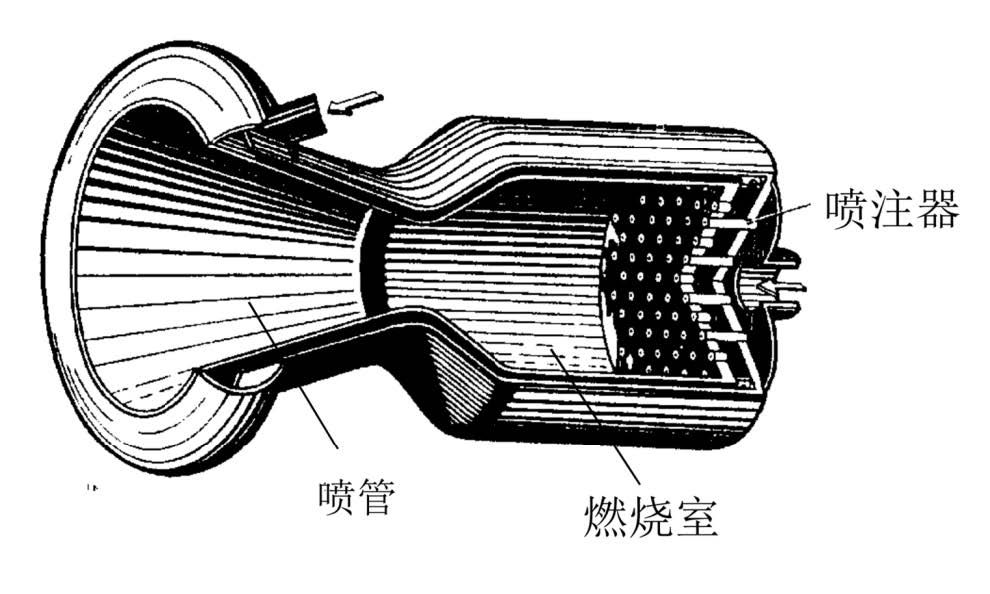
\includegraphics[width=\linewidth]{pic/推力室.jpg}
			\vspace*{-3em}
			\caption{推力室总体示意图}
			\label{推力室}
		\end{minipage}
		\begin{minipage}{0.45\linewidth}
			\centering
			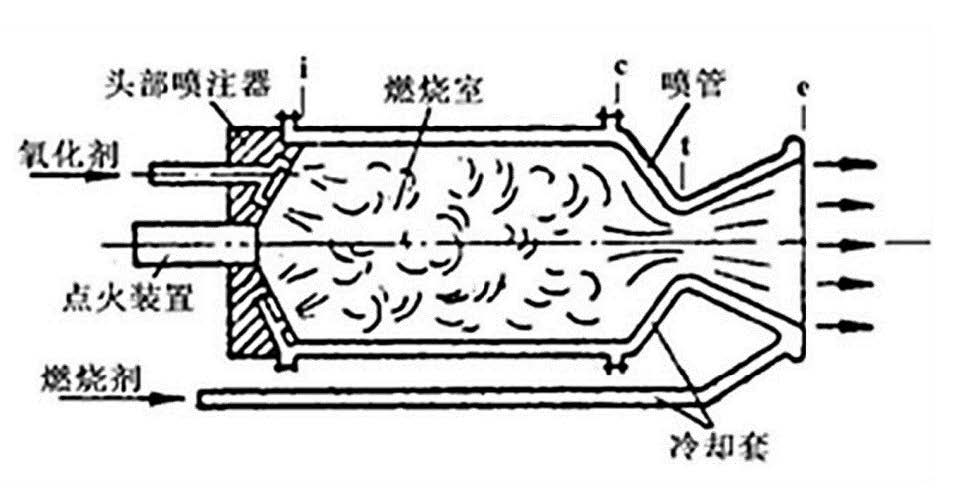
\includegraphics[width=\linewidth]{pic/推力室2.jpg}
			\vspace*{-2.8em}
			\caption{推力室内部示意图}
			\label{推力室2}
		\end{minipage}
	\end{figure}
	\vspace*{-1em}
	\item \textbf{工作过程} \hspace*{1em} 液体推进剂以\blue[规定的流量]和\blue[混合比]通过喷注器\blue[喷入燃烧室],在燃烧室内经过\blue[雾化、蒸发、混合和燃烧]等过程,产生的\blue[高温、高压燃气]在喷管内膨胀加速,以\blue[超声速]排出,从而产生推力。
	\item \textbf{特点} \hspace*{1em} \red[高温、高压环境],$3000\, \sim \, 4000 \degree\text{C}$,可以达到20$\,$MPa;\\
	\hspace*{3.5em}\red[化学反应速度很快,燃烧前准备过程决定燃烧速度]
\end{enumerate}

\sssection[推进剂供应系统]


\section{液体推进剂}
\subsection{液体推进剂分类及性能要求}
液体推进剂是翼液体状态进入推力室的推进剂,包括氧化剂和燃料以及单组元推进剂;可以是单质、化合物或混合物,是液体火箭发动机的能源和工质源,其质量占运载火箭起飞质量的70\% $\, \sim \,$90\%,直接影响着运载火箭和发动机的性能及制造费用。
\vspace*{0.5em}

\sssection[液体推进剂的分类]

\noindent \textbf{\underline{按进入推力室的基本组元数目分类}}
\vspace*{-0.5em}
\begin{enumerate}[\hspace*{1.5em} (1)  ]
	\item 单组元\\
	通过自身分解或燃烧能迅速产生高温高压的气体。\vspace*{-0.8em}
	\begin{enumerate}
		\item 在分子中同时含有可燃元素和燃烧所必需的氧的化合物,如:\underline{硝基甲烷、硝酸甲酯、过氧化氢} \vspace*{-0.5em}
		\item 在常压下互不产生化学反应的安定混合物,如:\underline{过氧化氢—甲醇}\vspace*{-0.5em}
		\item 在分解时能放出大量热量和气态产物的吸热化合物,如\underline{无水肼、甲基肼}\vspace*{-0.5em}
	\end{enumerate}
	单组元的特点:绝大多数单组元推进系统\blue[结构简单]、\blue[使用方便]、\blue[性能比较低]等\\
	单组元的应用:火箭发动机系统中的辅助能源,如涡轮泵燃气发生器、姿轨控制流
	
	\item 双组元\\
	由液体\red[燃烧剂]和\red[氧化剂]两种组员组成,工作时它们被分别从各自的贮箱和输送管路送入推力室。\vspace*{-0.8em}
	\begin{enumerate}
		\item 氧化剂:氧化力强的物质,如\underline{液氧、液氟、硝酸}等\vspace*{-0.5em}
		\item 燃烧剂(燃料):含氢量大、燃烧热值比较高的物质,如\underline{液氢、肼类、碳氢化合物}等\vspace*{-0.5em}
	\end{enumerate}
	双组元的特点:来源广泛、释放的能量较高\\
	双组元应用:液体火箭发动机绝大多数采用双组元推进剂
	
	\item 多组元
	由多于两组元组成的推进剂,常常指\dy[三组元]{SZY}。\vspace*{-0.8em}
	\begin{enumerate}
		\item 多于三组元的液体推进剂,理论上\red[能量不会进一步的增加]。\vspace*{-0.5em}
		\item 三组元足以能方便地把任何需要的化学元素组合起来。\vspace*{-0.5em}
	\end{enumerate}
	
	\item 三组元\vspace*{-0.8em}
	\begin{enumerate}
		\item 把轻金属(如锂、铍或铍的氢化物)同液氟、液氧或臭氧燃烧产生的高温与能够降低燃烧产物平均分子量的氢结合起来,提高比冲;\vspace*{-0.5em}
		\item 液氢、液氧和煤油 :在下面级工作时,常以氧为氧化剂、煤油为燃料并加入少量液氢燃料;\vspace*{-0.5em}
		\item 双燃料双膨胀:高压的内燃室中燃烧液氧、碳氢化合物;低压的外燃室燃烧液氧、液氢,带来起飞时高推力、小面积 比和高空的低推力、高面积比的优点。
	\end{enumerate}
\end{enumerate}

\noindent \textbf{\underline{按液体推进剂的贮存性能分类}}

\defination[地面可贮存推进剂]
{
	\dy[地面可贮存推进剂]{DMKZCTJJ} \quad 在\blue[相当宽的温度和压强范围]内、 在地面环境下能在贮箱内贮存一年或更长时间,不需外加能源加热熔化或冷却液化就能保持为液态又不变质的推进剂。多为硝基氧化剂、肼类、胺类和烃类燃料。
}
\noindent 具备条件:
\begin{enumerate}[\hspace*{1.5em}(1)  ]
	\item 临界温度不低于地面环境的最高温度\vspace*{-0.5em}
	\item 在323 K时的蒸气压不应大于2 MPa\vspace*{-0.5em}
	\item 在贮存期内,本身不分解变质、产生沉淀或放出气体\vspace*{-0.5em}
	\item 对与液体推进剂接触的部件不产生腐蚀。
\end{enumerate}

\defination[空间可贮存推进剂]
{
	\dy[空间可贮存推进剂]{KJKZCTJJ} \quad 在地面环境下不能贮存或难以贮存,但在空间环境下可以贮存的推进剂。其特点为其沸点低于空间环境温度,但高于200 K。
}

\noindent 空间不可贮存推进剂
\vspace*{-0.8em}
\begin{enumerate}[\hspace*{1.5em} (1) ]
	\item 低温推进剂\\
	定义:环境温度下是气体,沸点低于200 K,临界温度低于223 K,只有在低温才能保持为液态。\\
	特点:能量较高,使用不方便,有些价格昂贵;需要绝热措施和排气系统;液氧、液氢、液氟、二氟化氧及其某些混合物。\vspace*{-0.5em}
	
	\item 化学不稳定推进剂\\
	化学性质不稳定而只能在短期内使用。如,\underline{过氧化氢、叠氮化肼}。
\end{enumerate}

\noindent \textbf{\underline{按推进剂能量高低分类}}

\noindent 分类方法:采用一定的发动机工况(室压7 MPa、喷管出口截面出燃气压强0.1 MPa)时,发动机比冲大小。\vspace*{-0.5em}
\begin{enumerate}[\hspace*{1.5em} (1)  ]
	\item \dy[高能推进剂]{GNTJJ} \quad 比冲一般大于3000 m/s \vspace*{-0.5em}
	\item \dy[中能推进剂]{ZNTJJ} \quad 比冲在2500$\, \sim \,$3000 m/s之间 \vspace*{-0.5em}
	\item \dy[低能推进剂]{DNTJJ} \quad 比冲小于2500 m/s
\end{enumerate}

\noindent \textbf{\underline{按发动机用途分类}}

\dy[主推进剂]{ZTJJ}主要用于火箭、导弹等的主发动机

\dy[辅助推进剂]{FZTJJ}主要用于辅助发动机和发动机辅助系统

\vspace*{0.5em}

\noindent \textbf{\underline{按推进剂的自燃性质分类}}

\dy[自燃推进剂]{ZRTJJ}\quad 经简单混合后能自燃的推进剂

\dy[非自燃推进剂]{FZRTJJ} \quad 燃烧必需依靠外部提供能量,即需要点火装置


\sssection[发动机对液体推进剂对要求]

对液体推进剂对要求主要包括\underline{性能要求、使用要求、经济性要求}。
\vspace*{0.5em}

\noindent \textbf{\underline{性能要求}}\vspace*{-0.5em}
\begin{enumerate}[\hspace*{1.5em} (1) ]
	\item 高的比冲和高的密度\vspace*{-0.5em}
	\item 具有较高的热值\vspace*{-0.5em}
	\item 燃烧产物温度要高、分子量要低、燃烧产物不易解离、没有液态或固态产物存在
\end{enumerate}

\noindent \textbf{\underline{使用要求}}

要求液体推进剂的液态温度范围较宽、化学性质稳定且毒性小,对人员、设备和环境对污染小等。使用性能具体表现在
\vspace*{-0.5em}
\begin{enumerate}[\hspace*{1.5em} (1) ]
	\item \red[具有良好的运输型和输送性]\\
	粘度小其粘度随温度的变化率小;饱和蒸汽压小;推进剂中溶解的气体量少;所含悬浮颗粒物、粘性物质少
	\vspace*{-0.5em}
	
	\item \red[具有良好的点火和燃烧特性]\\
	着火延迟期(自燃推进剂)和点火延迟期不大于30 ms。
	
	\item \red[具有良好的冷却性能]
	\vspace*{-0.5em}
	
	\item \red[贮存稳定性好]\\
	与贮存材料相容性好;对空气和空气中的湿度不过于敏感;能经受环境温度的急剧变化。
	
	\item \red[具有良好的安全性能]\\
	热爆炸和热分解温度要搞;对机械冲击和突然压缩(水击)不敏感;无毒或低毒,燃烧产物对人和环境对毒害作用小。
\end{enumerate}

\noindent \textbf{\underline{经济型要求}}

原材料来源广泛、生产工艺简单、价格便宜。
\vspace*{0.5em}

\sssection[选择推进剂的原则]
\vspace*{-0.8em}
\begin{enumerate}[\hspace*{1.5em} (1)  ]
	\item 单位质量所释放的能量高、燃气的平均分子量要低 $\longrightarrow$ 确保高比冲\vspace*{-0.5em}
	\item 易于点火、燃烧稳定\vspace*{-0.5em}
	\item 密度大$\longrightarrow$较小推进剂贮箱和供应系统的尺寸和重量\vspace*{-0.5em}
	\item 高比热容、高热导率和高临界温度的最佳组合$\longrightarrow$可用作推力室的有效冷却剂\vspace*{-0.5em}
	\item 更低的饱和蒸汽压$\longrightarrow$利于泵的工作和设计\vspace*{-0.5em}
	\item 低冰点、高沸点 $\longrightarrow$ 发动机工作温度宽\vspace*{-0.5em}
	\item 无腐蚀性、毒性小 $\longrightarrow$ 与材料相容性好,对环境污染小\vspace*{-0.5em}
	\item 具有良好对可贮存性\vspace*{-0.5em}
	\item 低粘度 $\longrightarrow$ 易输送,通过供应系统和喷注器的压降小\vspace*{-0.5em}
	\item 高的热和冲击稳定性 $\longrightarrow$ 危险性小\vspace*{-0.5em}
	\item 低成本
\end{enumerate}
\vspace*{0.5em}

\subsection{液体推进剂物理化学参数}


\section{液体火箭发动机系统及工作}
\subsection{挤压式推进剂供应系统}
\noindent \textbf{\underline{推进剂供应系统}}

\blue[功能]\quad 将贮箱中的推进剂按照要求的流量和压强输送到推力室中。

\blue[分类]\quad 按其工作的方式,可分为挤压式和泵压式两大类。
\vspace*{0.5em}

\clearpage
\begin{minipage}{0.5\linewidth}
	\noindent \textbf{\underline{挤压式推进剂供应系统}}
	
	\blue[原理]\quad 利用高压气体将液体推进剂挤压出来输送到推力室;
	
	\blue[优缺点]\quad 简单、可靠;较高压强下结构比较笨重;
	
	\blue[适用性]\quad 小推力、工作时间较短;
	\vspace*{0.8em}
	
	\blue[组成]  \quad 
	$
	\begin{cases}
		\, \mbox{推进剂贮箱}\\
		\, \mbox{用来建立供应压强的气源}\\
		\, \mbox{各种功能的阀门}\\
		\, \mbox{参数调节或校准元件}\\
		\, \mbox{导管和其他附件}
	\end{cases}
	$
\end{minipage}
\begin{minipage}{0.5\linewidth}
	\centering
	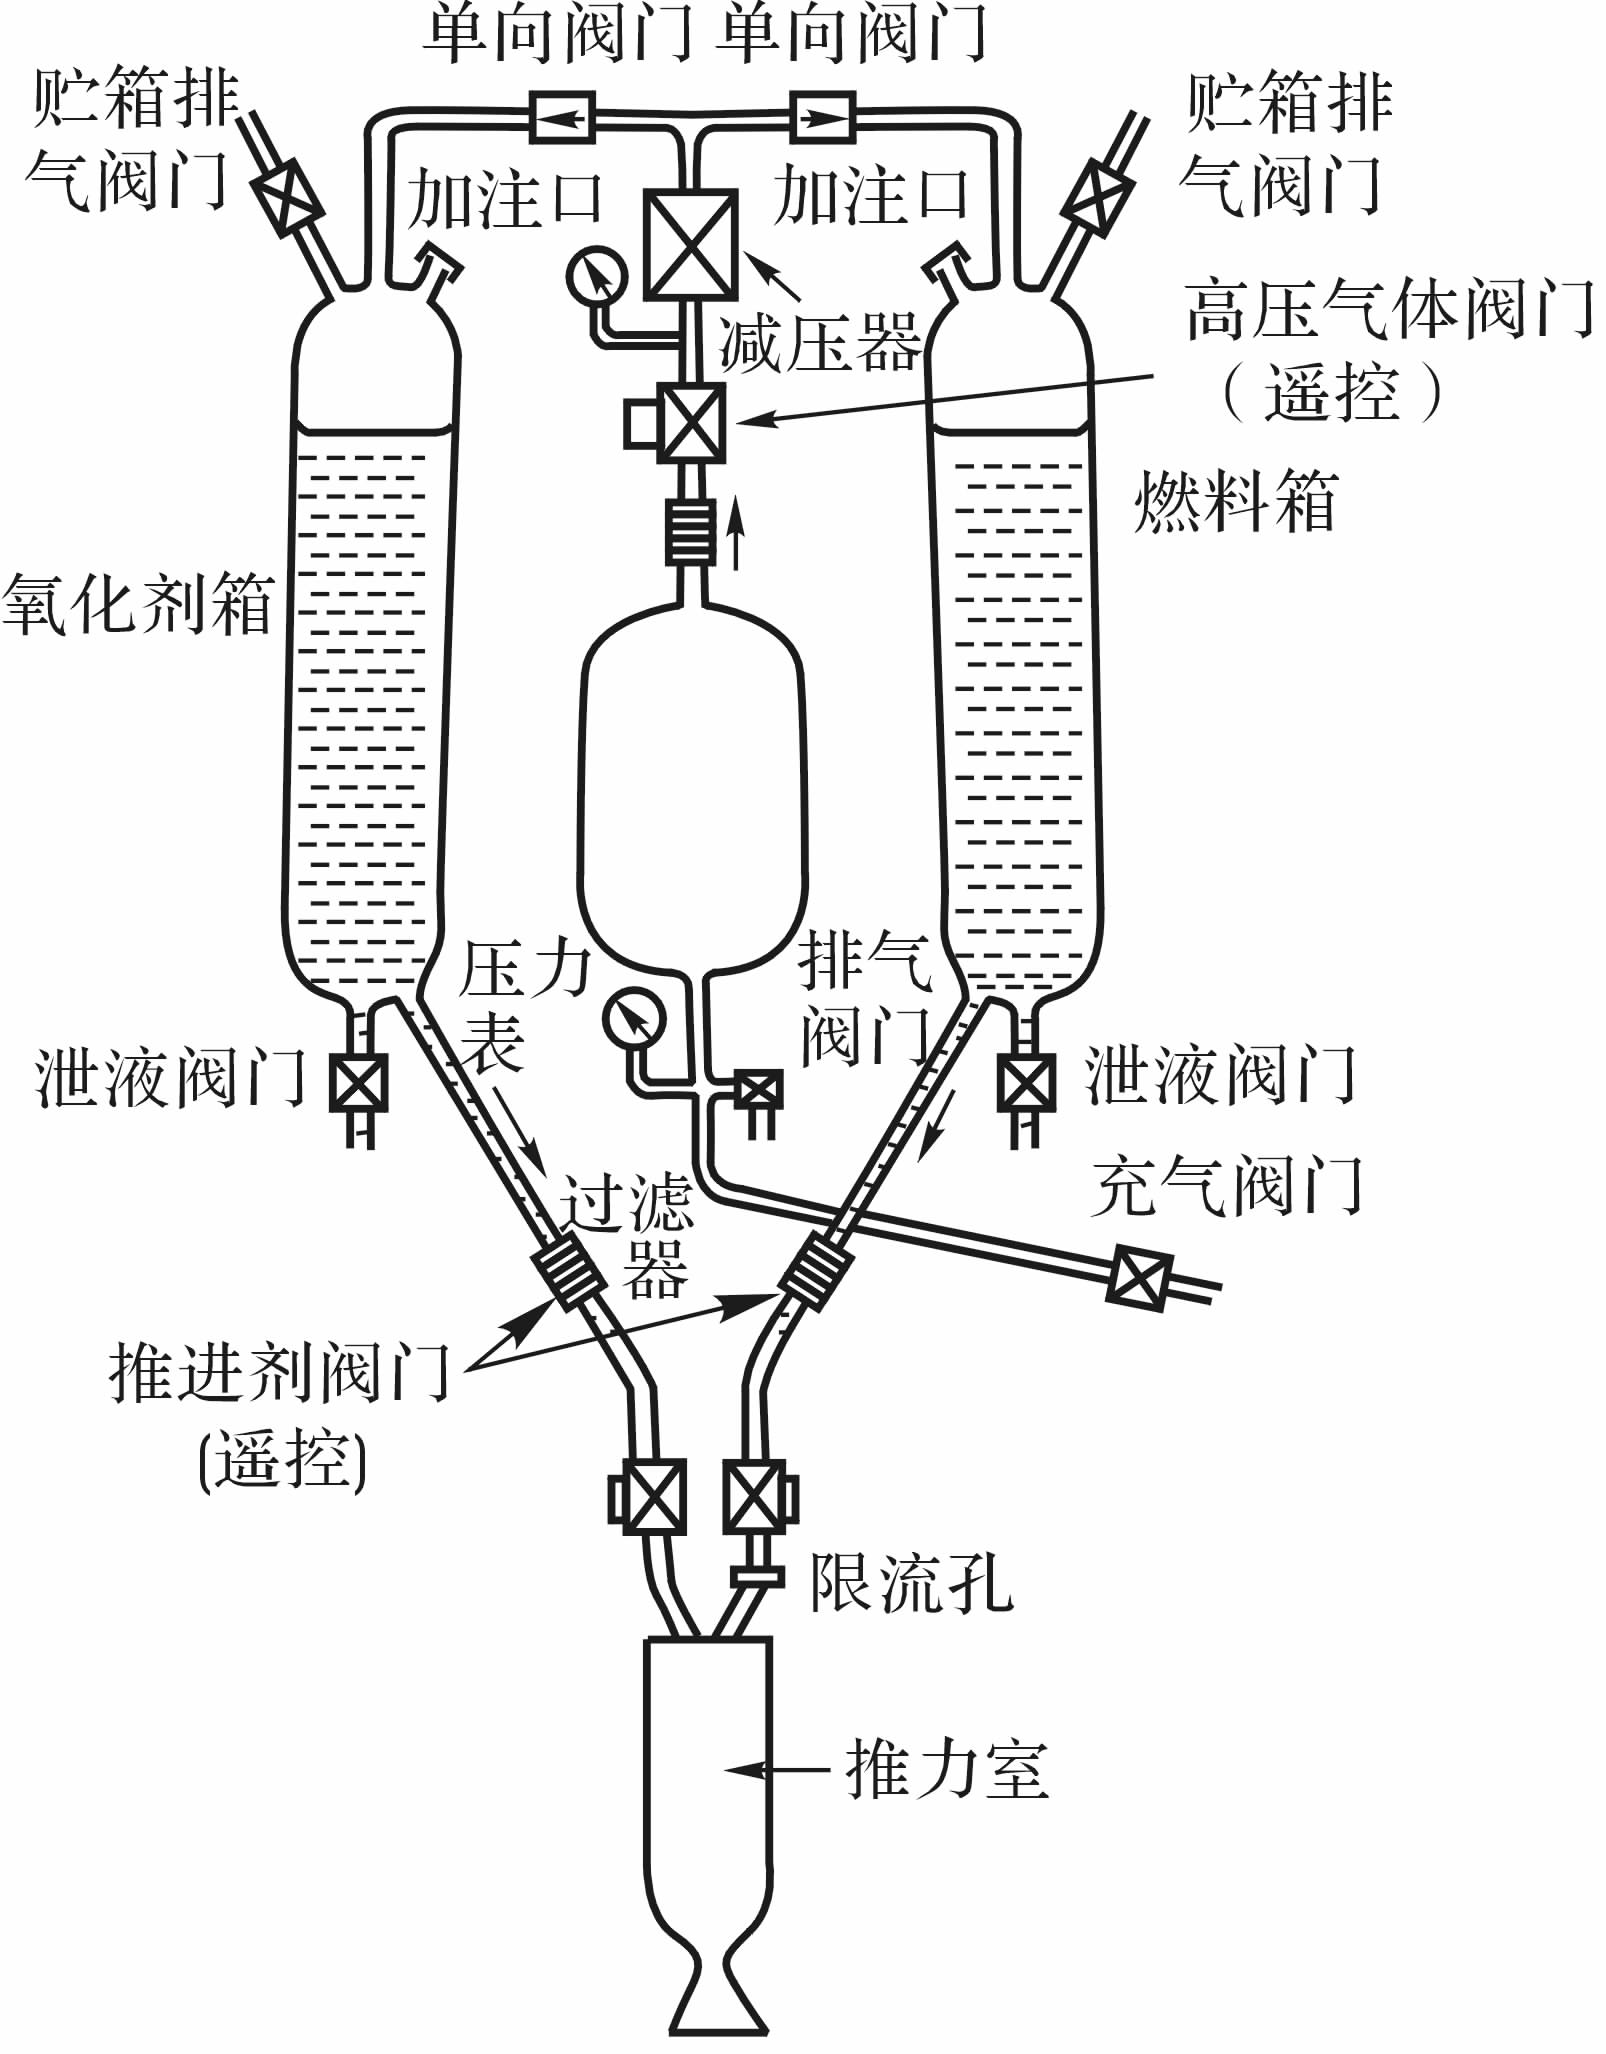
\includegraphics[width=0.8\linewidth]{pic/气压.png}
	\captionof{figure}{气体挤压式推进剂供应系统}
\end{minipage}


\vspace*{0.8em}
\noindent
\begin{minipage}{0.6\linewidth}
	\sssection[挤压式供应系统分类]
	
	\blue[对挤压工质的要求]\quad 与推进剂有良好的\red[相容性] ;最小的分子量具有适当的温度,且热稳定性要好。
	
	挤压气源是来自高压气瓶,瓶内压强约为20$\, \sim \,$35 MPa ,通过降压方式到工作压强。按照降压方式,又分为减压器降压式和直接膨胀降压式。
	\vspace*{0.8em}
	
	\sssection[冷气体挤压]
	\vspace*{-0.8em}
	\begin{enumerate}[\hspace*{1.5em} (1) ]
		\item \textbf{气瓶式(或贮气式)冷气挤压}\\
		\blue[常用挤压气体] \quad 空气、氮气和氦气。对于低温推进剂,空气和氮气遇冷后会发生凝结,应选用氦气。\vspace*{-0.5em}
		
		\item \textbf{蒸发系统汽化式}\\
		挤压气源是利用液体的汽化而得到。\\[0.5em]
		按照使用液体的来源,分为推进剂蒸发系统和非推进剂蒸发系统,即将容易气化的推进剂组元或非推进剂液体通过换热器加热、气化后去挤压贮箱中的推进剂。
		\begin{equation*}
			\begin{cases}
				\, \mbox{\blue[推进剂蒸发系统]}\quad \mbox{仅适用于热稳定的低沸点推进剂,如氢;(注:也适用泵式发动机)}\\
				\, \mbox{\blue[非推进剂蒸发系统]} \quad \mbox{主要是惰性气体蒸发系统,如液氮、液氦}
			\end{cases}
		\end{equation*}
	\end{enumerate}
\end{minipage}
\begin{minipage}{0.4\linewidth}
	\centering
	\vspace*{-4em}
	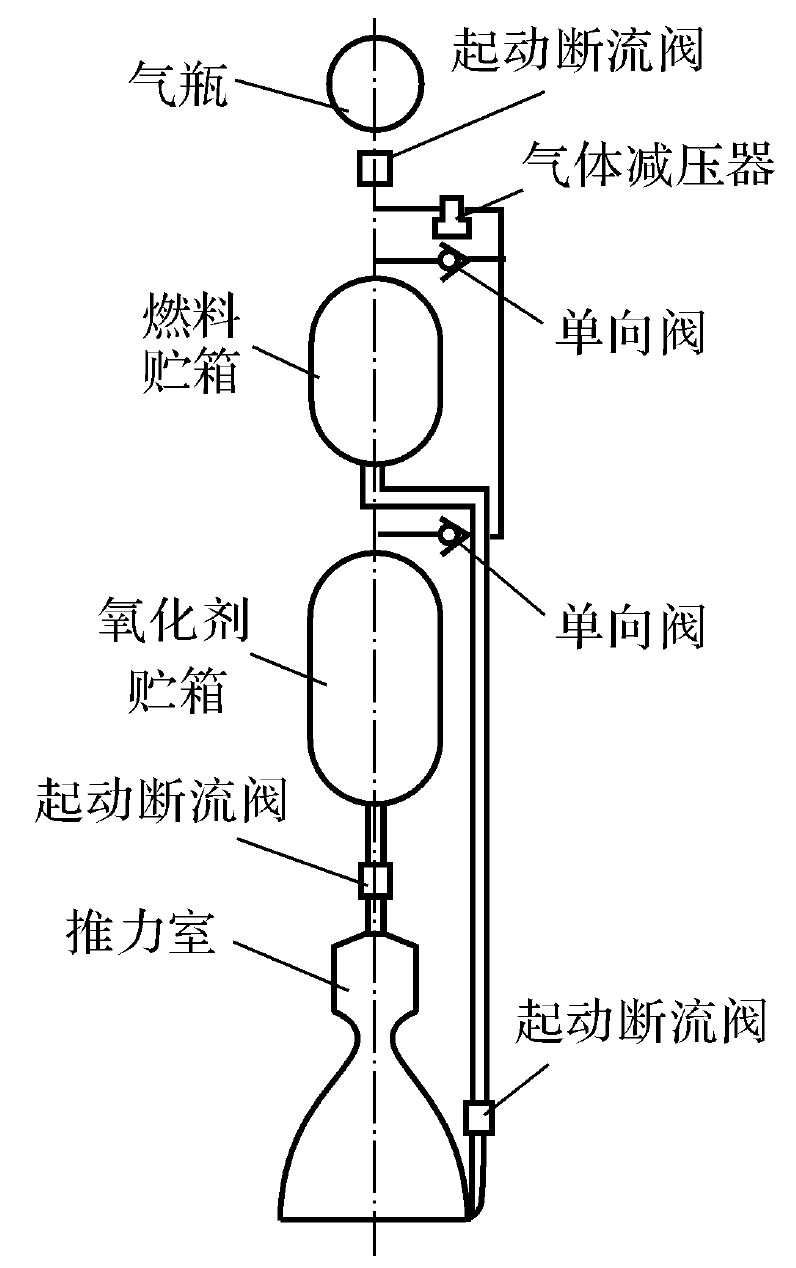
\includegraphics[width=0.8\linewidth]{pic/气瓶挤压.png}
	\vspace*{-1em}
	\captionof{figure}{气瓶式挤压式推进剂供应系统}
\end{minipage}

\vspace*{1em}
\sssection[热气体挤压]

\blue[适用范围] \quad 不能应用于低温推进剂:产物中的水会凝结吸热,会提高低温推进剂的温度。
\vspace*{0.5em}

\blue[分类]\quad 按产生热挤压气体的途径分类:
$
\begin{cases}
	\, \mbox{燃气发生器式}\\
	\, \mbox{化学反应式}
\end{cases}
$

\begin{enumerate}[\hspace*{1.5em} (1) ]
	\item \textbf{燃气发生器}\\
	按使用推进剂分类:
	\vspace*{-0.5em}
	\begin{enumerate}
		\item 固体燃气发生器\\
		基本组成\quad 固体推进剂燃气发生器(壳体、药柱、点火器)、过滤器和燃气调节装置及冷却热燃气的装置(不是必须)等。
		\begin{table}[!htb]
			\centering
			\setlength{\tabcolsep}{14mm}{
			\begin{tabular}{cl}
				\toprule
				固体燃气发生器类型 & 基本原理\\
				\midrule
				\makecell[c]{无冷却的\\固体燃气发生器} & \makecell[l]{固体燃气发生器产生燃气;\\过滤器过滤燃气;\\调节器排出多余燃气。}\\
				\hline
				 \makecell[c]{使用固体冷却剂的\\燃气发生器
} &\makecell[l]{推进剂:硝酸铵基;  冷却剂:粒状的草酸。 \\热燃气通过固体冷却剂冷却升华\\或分解产生附加的挤压气体($\text{CO}_2, \text{H}_2\text{O}, \text{CO}$)。}\\
				 \hline
				 \makecell[c]{使用叠氮化物冷却的\\燃气发生器} & \makecell[l]{热燃气通过叠氮化物冷却层被冷却,\\叠氮化物分解并产生氮气;\\但燃气中含有金属粒子,要用旋转分离除去。\\能提供较纯的氮气。
				 }\\
				 \hline
				 \makecell[c]{使用燃气发生器\\加热的氮气系统
} & \makecell[l]{固体燃气发生器安装在氦气瓶内,\\提供热量和 附加的挤压气体。
}\\
				\bottomrule
			\end{tabular}
		}
		\end{table}
	
	\begin{figure}[!htb]
		\begin{minipage}{0.25\linewidth}
			\centering
			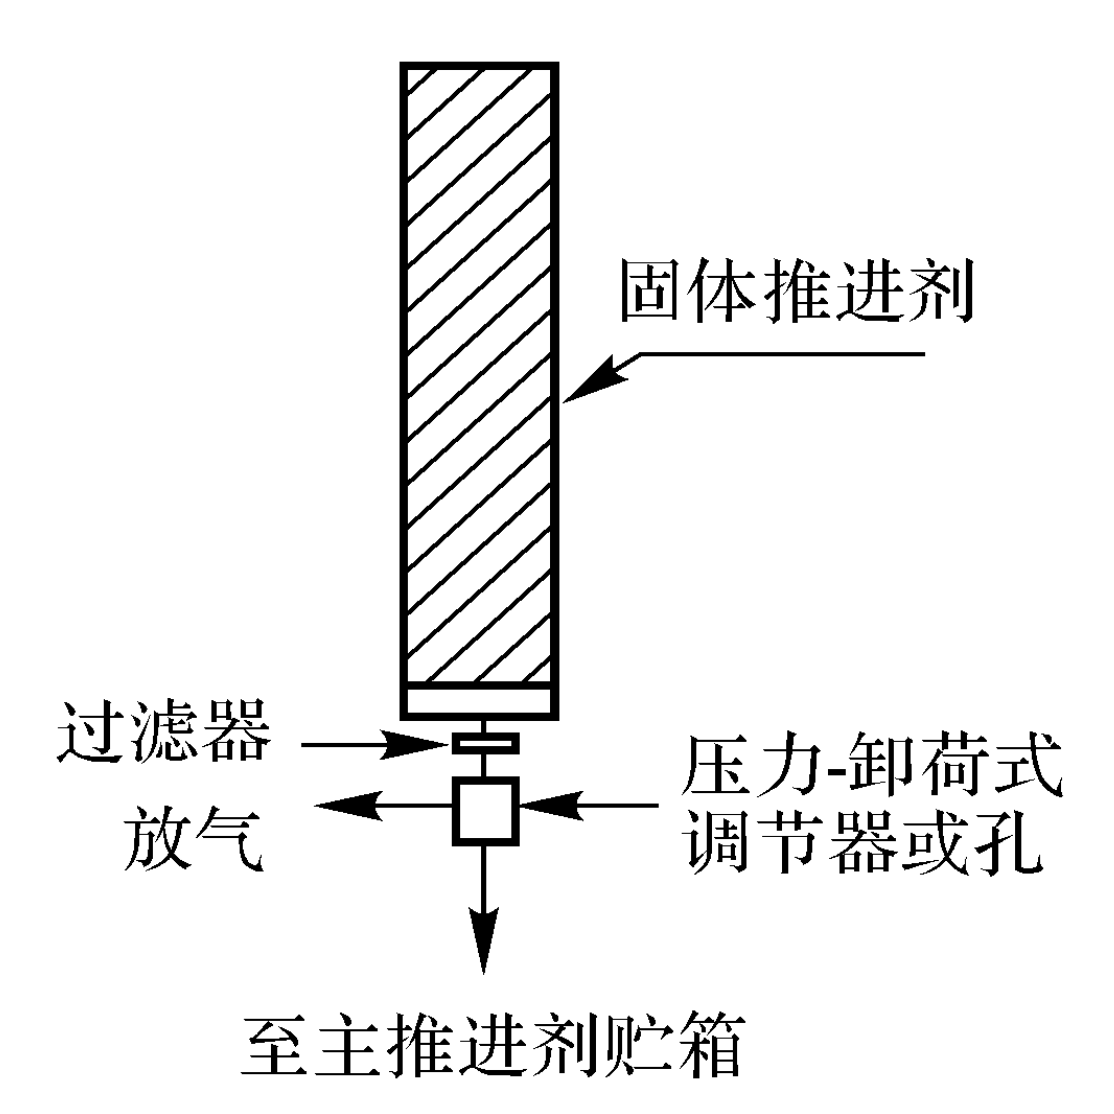
\includegraphics[width=\linewidth]{pic/固体1.png}
		\end{minipage}
		\begin{minipage}{0.25\linewidth}
			\centering
			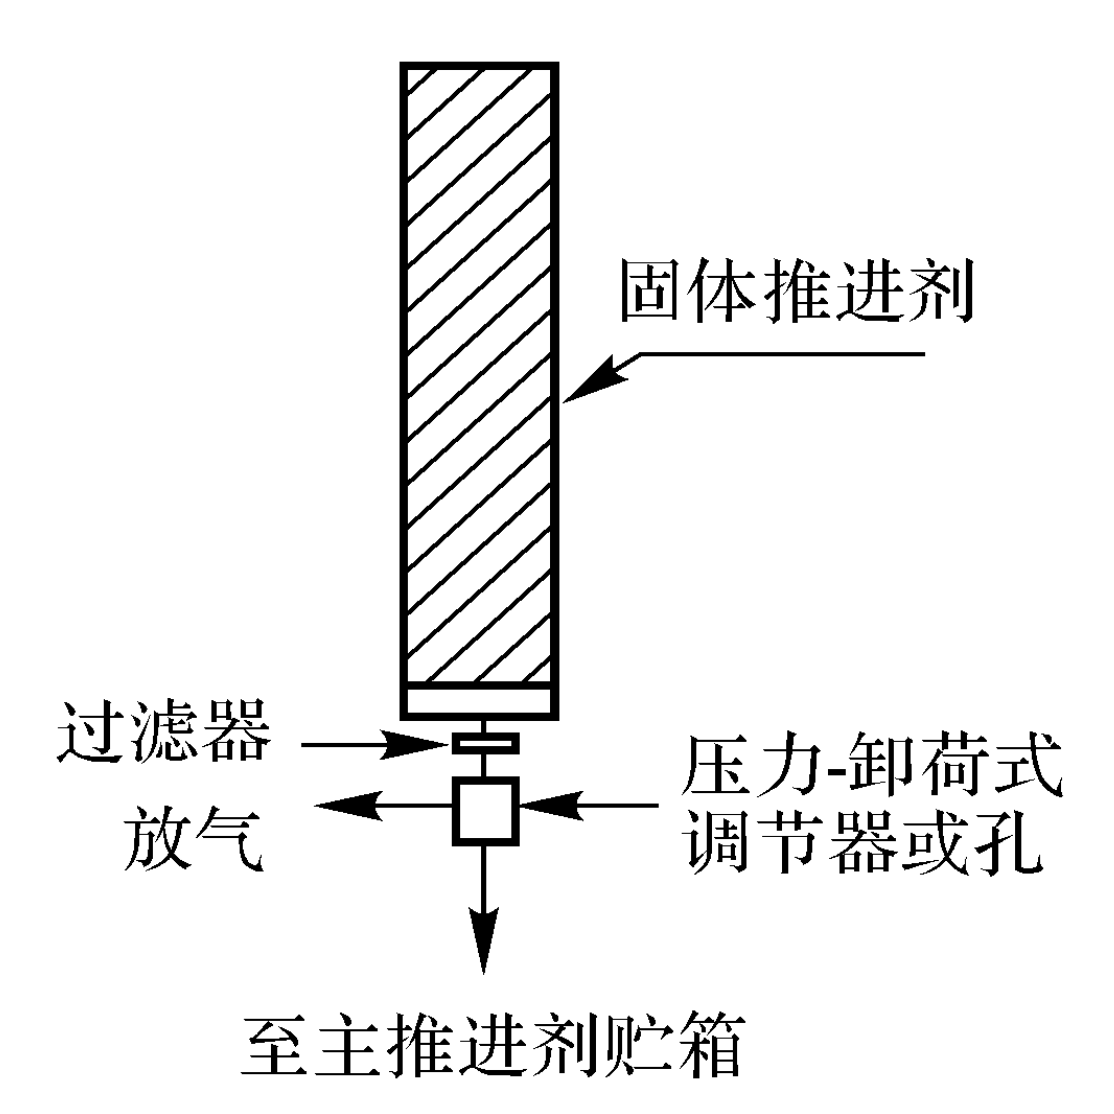
\includegraphics[width=\linewidth]{pic/固体1.png}
		\end{minipage}
		\begin{minipage}{0.25\linewidth}
			\centering
			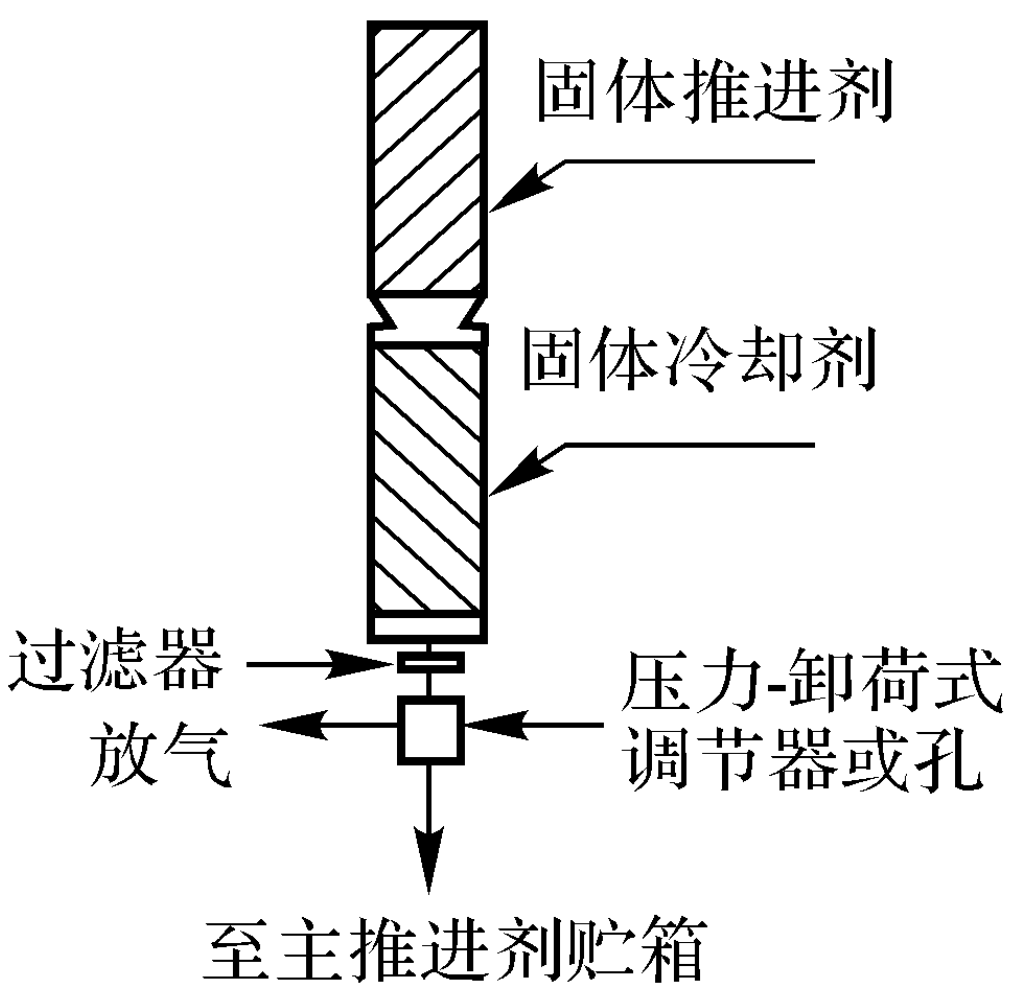
\includegraphics[width=\linewidth]{pic/固体3.png}
		\end{minipage}
		\begin{minipage}{0.20\linewidth}
			\centering
			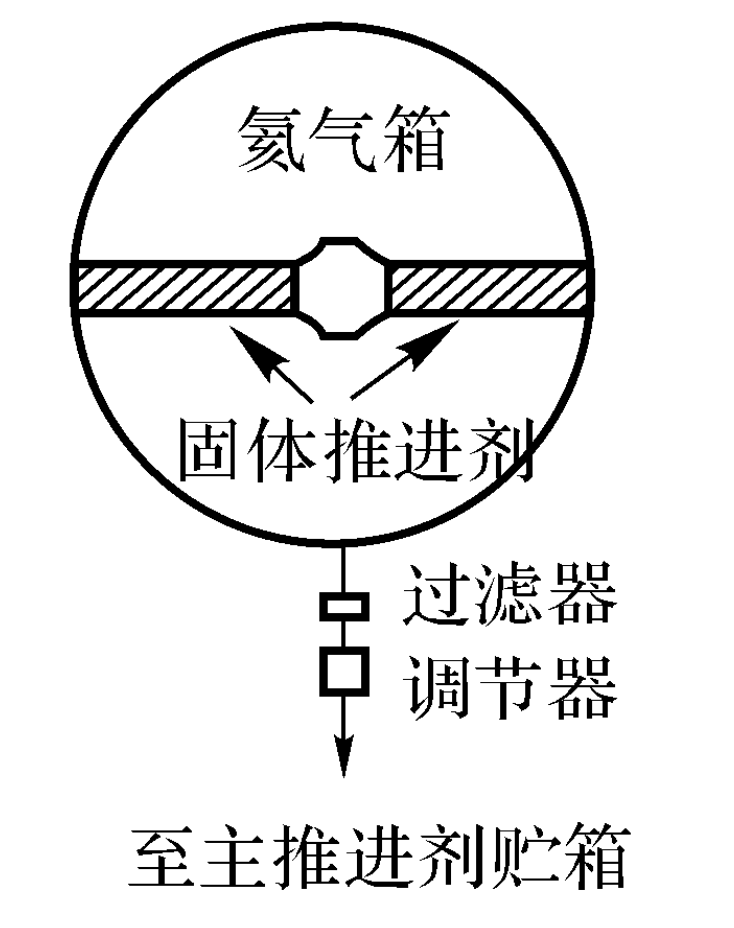
\includegraphics[width=\linewidth]{pic/固体4.png}
		\end{minipage}
	\caption{四种固体燃气发生器类型}
	\end{figure}
	
	\item 液体燃气发生器
	\begin{table}[!htb]
		\centering
		\setlength{\tabcolsep}{10mm}{
			\begin{tabular}{cl}
				\toprule
				液体燃气发生器类型 & 基本原理\\
				\midrule
				\makecell[c]{具有喷注冷却的\\单燃气发生器} & \makecell[l]{单组元$+$不反应的冷却剂, 产生低温燃气;\\
				双组元,使混合比远远偏离化学当量比,产生低温燃气。}\\
				\hline
				\makecell[c]{具有单个燃气\\发生器的氦气系统
} &\makecell[l]{燃气发生器通过换热器加热氦气,\\用热氦气其挤压 氧化剂贮箱;
\\燃气挤压主燃料贮箱。}\\
				\hline
				\makecell[c]{具有喷注冷却的\\两个双组元燃气发生器} & \makecell[l]{用氦气挤压两个辅助推进剂贮箱,供应燃气发生器;
\\富燃燃气发生器产生的燃气挤压主燃料贮箱;\\
富氧的燃气发生器产生的燃气挤压主氧化剂贮箱。}\\
				\bottomrule
			\end{tabular}
		}
	\end{table}
	
	典型的双组元液体燃气发生器式挤压系统如图\ref{双组元}所示。
	\end{enumerate}
	
	\begin{figure}[!htb]
		\centering
		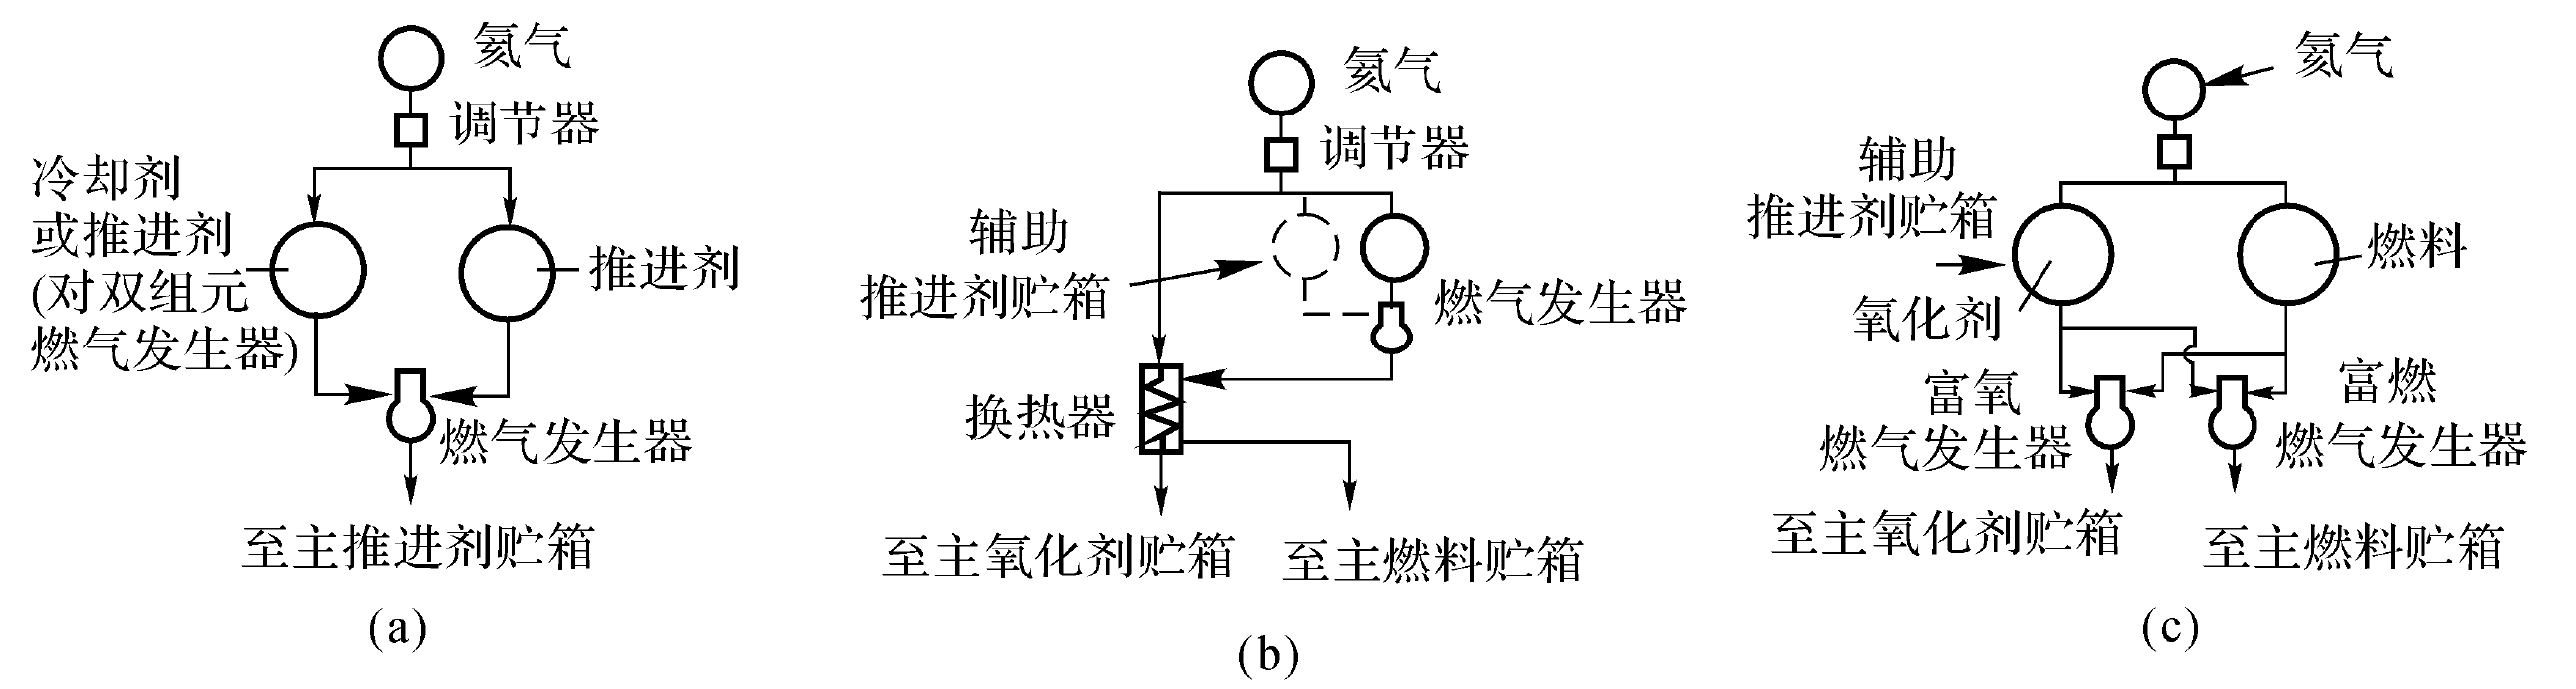
\includegraphics[width=0.9\linewidth]{pic/液体.png}
		\caption{三种液体燃气发生器类型}
	\end{figure}
	
	\begin{figure}[!htb]
		\centering
		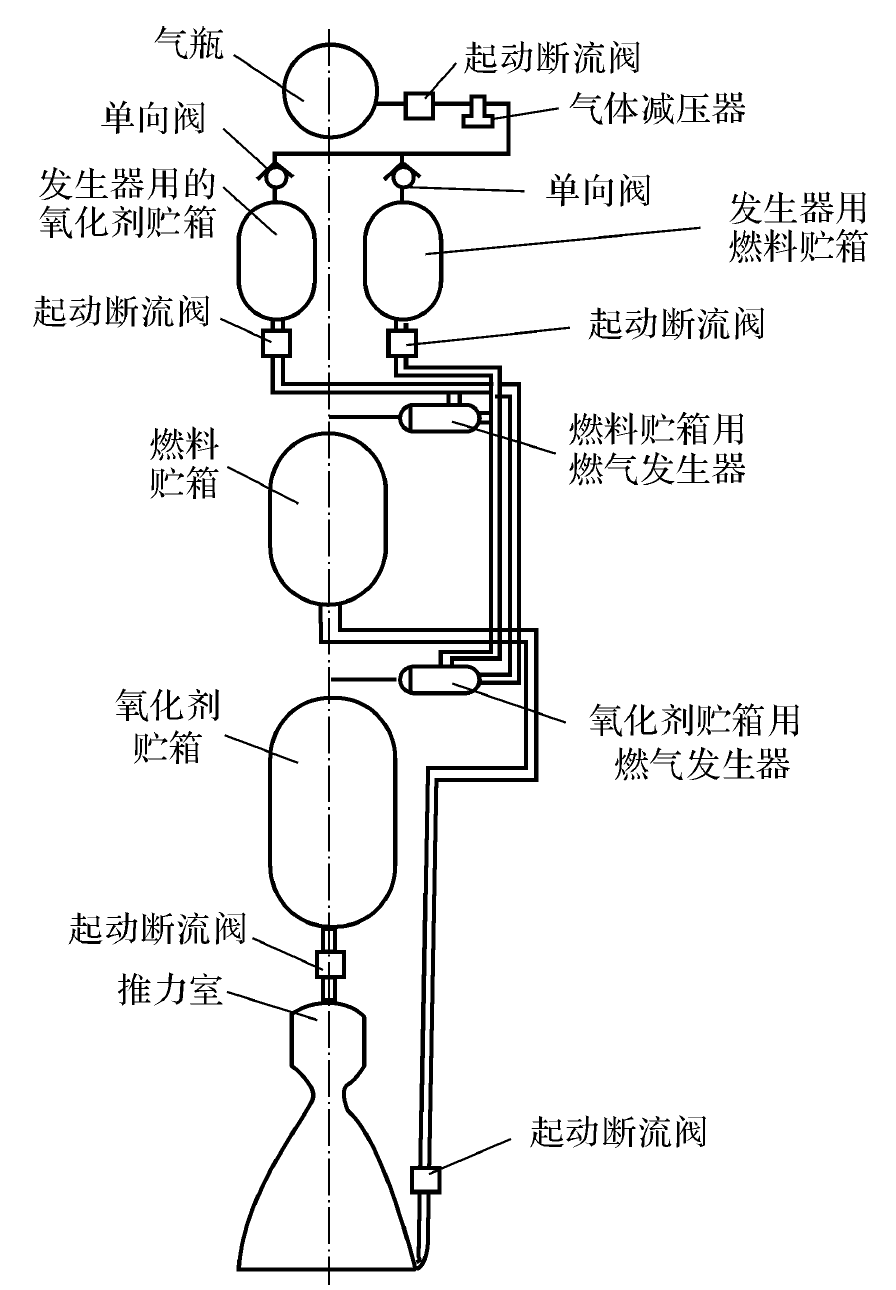
\includegraphics[width=0.35\linewidth]{pic/双组元液体.png}
		\caption{双组元液体燃气发生器式挤压系统}
		\label{双组元}
	\end{figure}
	
	\item \textbf{化学反应式}\\
	在贮箱中直接发生化学反应,即将少量燃料喷注到氧化剂贮箱中,或
将少量氧化剂喷注到燃料贮箱中,发生化学反应,从而产生挤压气体。
有两种类型:
	\vspace*{-0.5em}
	\begin{itemize}
		\item \blue[双直接喷注式]\quad 两个辅助贮箱。
		\item \blue[串联直接喷注式]\quad 一个辅助贮箱;在系统安全、可靠性和 调节贮箱稳态压力等方面存在设计问题。
	\end{itemize}
	\begin{figure}[!htb]
		\centering
		\subfigure[双直接喷注式]{
		\begin{minipage}{0.4\linewidth}
			\centering
			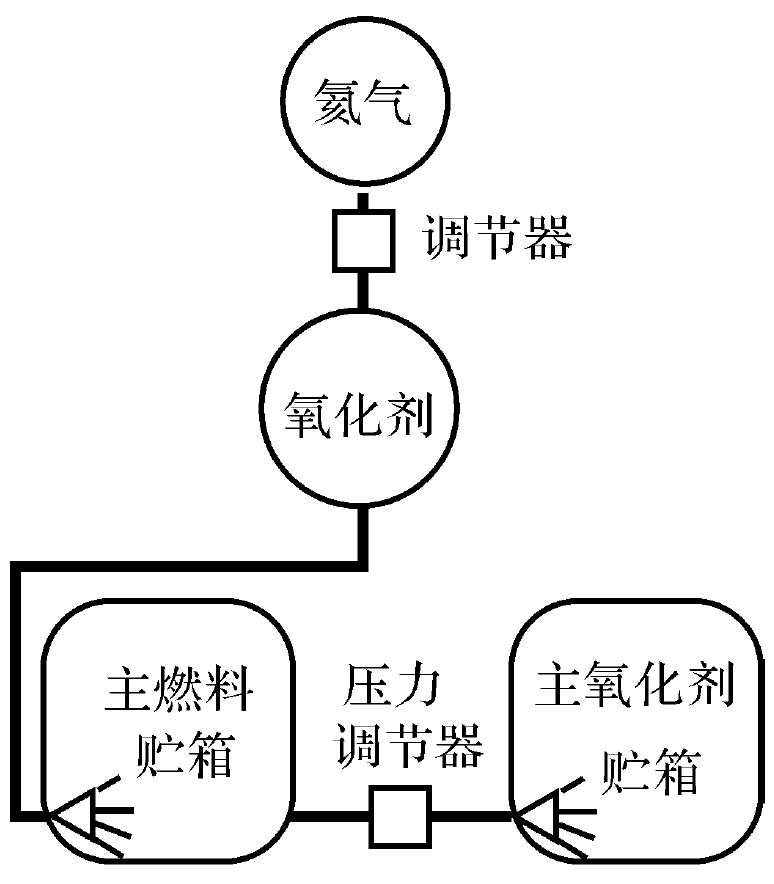
\includegraphics[width=0.5\linewidth]{pic/化学1.png}
			\vspace*{0.5em}
		\end{minipage}
		}
		\subfigure[串联直接喷注式]{
		\begin{minipage}{0.4\linewidth}
			\centering
			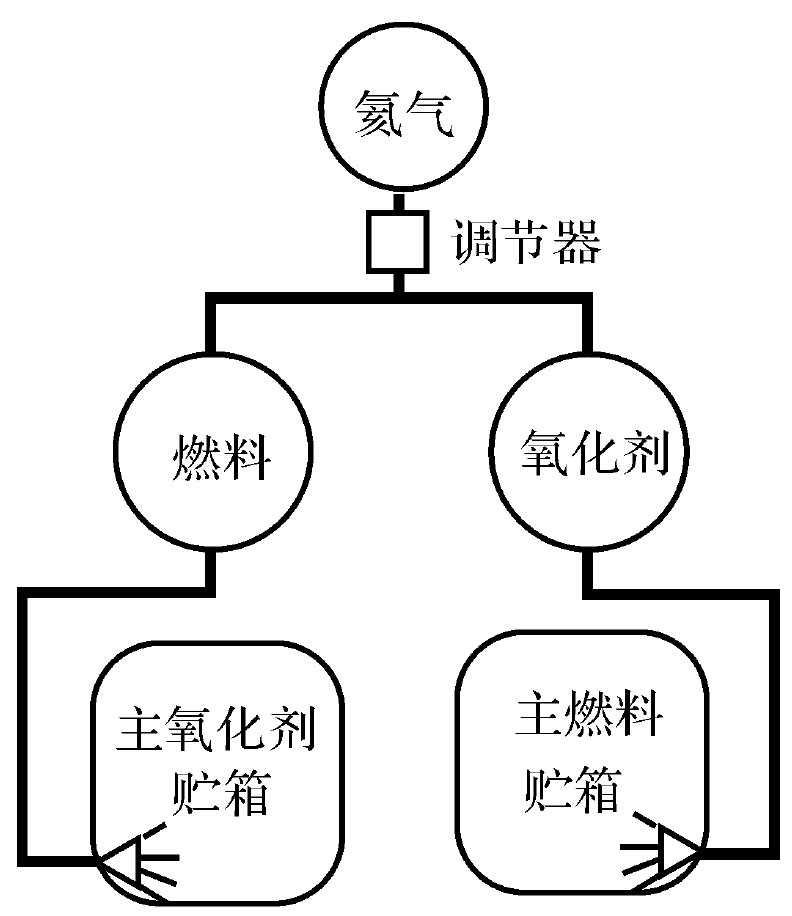
\includegraphics[width=0.5\linewidth]{pic/化学2.png}
			\vspace*{0.5em}
		\end{minipage}
	}
	\caption{化学反应式挤压系统}
	\vspace*{-2em}
	\end{figure}
\end{enumerate}

\sssection[各种挤压系统的对比]
\begin{table}[!htb]
	\centering
	\setlength{\tabcolsep}{2.5mm}{
	\begin{tabular}{m{0.1\textwidth}<{\centering} m{0.25\textwidth}<{\centering} m{0.25\textwidth}<{\centering} m{0.28\textwidth}<{\centering}}
		\toprule
		类别 & 气瓶贮气系统 & 液体蒸发系统 & 热气挤压系统 \\
		\midrule
		优点 & 结构简单,技术成熟 & 辅助气瓶和辅助贮箱尺寸小系统结构质量小 & 辅助气瓶和辅助贮箱尺寸小,系统结构质量小固体发生器系统结构简单\\
		\hline
		缺点 & 气瓶容积大,系统质量大 & 需要辅助气瓶、辅助贮箱和换热器,结构复杂 & 对液体发生器和在贮箱中直接化学反应的系统,结构复杂;固体发生器系统不能多次起动\\
		\hline
		适用范围 & 总冲量比较小的发动机 & 热稳定、低沸点的推进剂组元,若推进剂都不易汽化,可以选用液化气体 & 常温推进剂\\
		\bottomrule
	\end{tabular}
}
\end{table}

\noindent \textbf{\underline{挤压系统的选择}}

\par (1) \hspace*{0.5em}\red[任务和运载器的要求。]包括贮存性能、系统的起动和再起动以及压强和流量的精度等。
\par (2) \hspace*{0.5em}\red[挤压气体与推进剂、贮箱材料的相容性。] 包括化学惰性、过凝结和过溶解气体产物的防止以及适当的挤压物质温度。
\par (3) \hspace*{0.5em}\red[挤压式系统的可靠性。] 可靠性是在系统复杂性和失效模式的基础上估计的,应大力发展可靠性高的组件,包括燃气发生器、换热器和调节器等。
\par (4) \hspace*{0.5em}\red[成本。]
\par (5) \hspace*{0.5em}\red[挤压式系统的重量和尺寸。]

挤压系统的\blue[特点]:技术成熟,可靠性高;系统比较笨重。\blue[适用于]小推力或工作时间较短的火箭发动机。
\vspace*{0.5em}

\subsection{泵压式推进剂供应系统}

\begin{figure}[!htb]
	\centering
	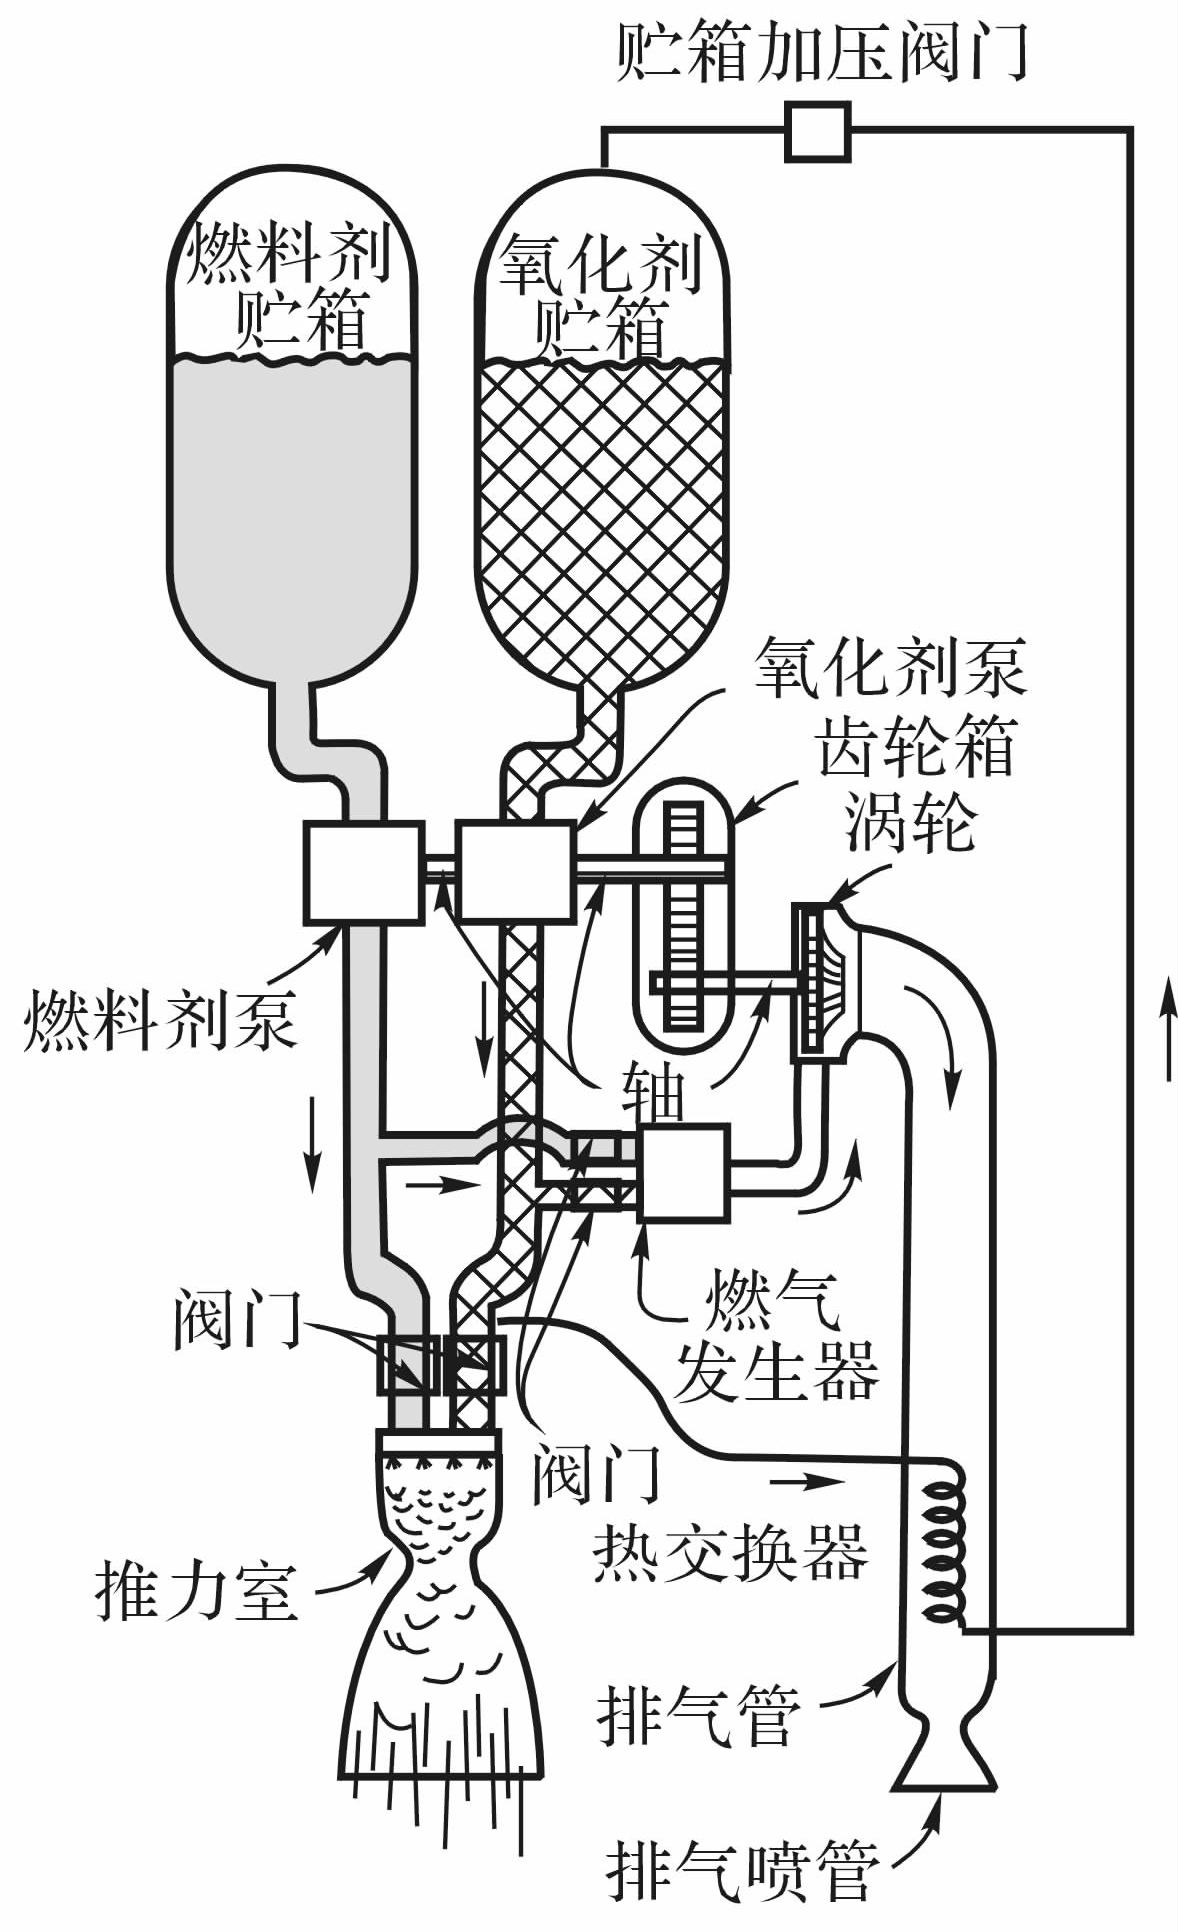
\includegraphics[width=0.3\linewidth]{pic/泵压.png}
	\caption{泵压式推进剂供应系统}
\end{figure}

\defination[泵压式供应系统]
{
	\blue[原理]\quad 利用涡轮泵将推进剂从贮箱中抽出、增压,输送至推力室;\\
	\hspace*{2em} \blue[关键部件]\quad 涡轮泵\\
	\hspace*{2em} \blue[特点]\quad 泵前推进剂是低压,贮箱结构质量可以较轻,一般$\le 0.5\,$MPa.\\
	\hspace*{2em} \blue[适用]\quad 工作时间长的大中型液体发动机。
}




















	
	%打印索引—————————————
	\cleardoublepage
	\addcontentsline{toc}{chapter}{附录}
	\addcontentsline{toc}{section}{索引}
	\color{titlepurplec}
	\appendix
	\printindex
	%———————————————
	
\end{document}